\documentclass[12pt,a4paper]{book}
%% Packages élémentaires %%
\usepackage[utf8]{inputenc}
\usepackage{mathpazo,etoolbox, graphicx, wrapfig, pbox, fancybox, hyperref, appendix, geometry, amsmath, amssymb, tikz, pgfplots, calc, enumitem}
\graphicspath{{images/}}
\geometry{hmargin=2.4cm, vmargin = 2.1cm}
\setlist[itemize]{itemsep=10pt, label={--}}

%% Couleurs %%
\usepackage{xcolor}
\definecolor{bleu}{RGB}{14, 68, 175}
\definecolor{bleu3}{RGB}{222, 233, 255 }
\definecolor{orange2}{RGB}{255, 216, 154}
\definecolor{rouge}{RGB}{201, 0, 0}
\definecolor{vert}{RGB}{14, 137, 0}
\definecolor{gris}{RGB}{222,230,230}
\newcommand\rouge[1] {{\color{rouge}{#1}}}
\newcommand\bleu[1] {{\color{bleu}{#1}}}
\newcommand\green[1]{{\color{vert}{#1}}}


%% Cadres %%
\newcommand\bb[1]{
\begin{center}
\fcolorbox{black}{bleu3}{\parbox{\textwidth}{ 
#1
}}
\end{center}}

\newcommand\boite[1]{
\begin{center}
\fbox{\parbox{\textwidth}{ \begin{center}
\begin{Large}
#1
\end{Large}
\end{center}}}
\end{center}}

\newcommand\aparte[1]{
\begin{center}
\fcolorbox{white}{gris}{\parbox{\linewidth}{ \textit{A parte} \\
#1 }}
\end{center}}

\newcommand\exemple[1]{
\begin{center}
\fcolorbox{white}{gris}{\parbox{\linewidth}{ \textit{Exemple} \\
#1 }}
\end{center}}

%% Commandes %%
\newcommand\imp[1]{\underline{\textbf{#1}}}
\newcommand\eq[1]{\begin{large}
\begin{align*}
#1
\end{align*}
\end{large}}
%% Commandes fantaisistes (cf. Internet) %%
\renewcommand{\parallel}{ \mathbin{\!/\mkern-5mu/\!} }
\newcommand{\q}[1]{{%
\font\larm = larm1000%
\larm%
\char 190}{ \textit{#1} }{%
\font\larm = larm1000%
\larm%
\char 191}}

%% Wrapping %%
\newcommand\wrap[4]{\begin{wrapfigure}[#1]{#2}{#3\textwidth}
#4
\end{wrapfigure}}

\usepackage[french]{babel}
\usepackage{algorithm, algorithmic}
\title{Compléments d'algorithmique}
\author{Sami \textsc{Abdul Sater}}
\graphicspath{{images/}}

\newcommand{\divc}{\textit{divide-and-conquer} }
\newcommand{\pseudo}[1]{\rouge{\textsc{#1}}}
\floatname{algorithm}{Procedure}
\begin{document}
\maketitle
\tableofcontents
\chapter{Introduction}
\section{Algorithme}
Un \textbf{algorithme} est une méthode de calcul qui, à partir d'un ensemble de valeurs d'entrée, permet d'obtenir des valeurs de sortie répondant à un problème donné (et pour lequel l'algorithme a été conçu). \\

\subsection{Instance d'un problème}
L'objectif  de conception d'un algorithme est qu'il puisse résoudre un problème pour toute valeur d'entrée. De manière plus rigoureuse, on applique en réalité un algorithme à une \textit{instance d'un problème} : il s'agit de l'ensemble des valeurs d'entrée. La sortie consiste donc en la solution de cette instance du problème. 

\bb{Un algorithme doit donc être capable de résoudre toutes les instances du problème pour lequel il a été conçu.}

\subsection{Lien entre algorithme et programme}
Un programme est simplement la transcription d'un algorithme pour un ordinateur. Là où les programmes que nous connaissons sont écrits avec un langage de programmation compréhensible par une machine (après compilation), les algorithmes sont \textbf{écrits en pseudo-code} et sont en général pas écrits pour un ordinateur mais, pour rester inclusif, pour un \textbf{modèle de calcul}. C'est l'analogue de l'ordinateur pour les programmes.

\begin{table}[h]
\centering
\begin{tabular}{r|l}
     \bleu{Programme} & \rouge{Algorithme} \\ \rule{0pt}{20pt}
     \bleu{Langage de programmation} & \rouge{Pseudo-code} \\ \rule{0pt}{20pt}
     \bleu{Ordinateur} & \rouge{Modèle de calcul}
\end{tabular}
\caption{Comparaison entre programme et algorithme}
\label{tab:algo_prog}
\end{table}
\subsection{Modèle de calcul -- machine RAM}
Le modèle de calcul sur lequel vont être appliqués nos algorithmes va être la \textbf{machine RAM} : il s'agit d'une machine à "accès aléatoire", c'est-à-dire qui nous donne accès à une mémoire de grande taille, sur laquelle nous pourrons effectuer nos opérations. Nous distinguons alors naturellement les instructions \textbf{élémentaires} des instructions \textbf{non-élémentaires} qui sont constituées d'instructions élémentaires.
\begin{itemize}
\item Élémentaires : lecture d'une donnée du tableau, écrire une valeur dans le tableau, instructions arithmétiques (addition, multiplication ...), de test (égalité, superiorité), et logiques (négation, et, ou).
\item Non-élémentaires : tout le reste ! Par exemple, une insertion est non-élémentaire parce qu'il faut décaler les données avant d'insérer.
\end{itemize}

\subsection{Qualités d'un algorithme}
Nous nous attendons d'un algorithme :
\begin{itemize}
\item Qu'il se termine en un temps fini 
\item Qu'il soit efficace : qu'il y ait le moins d'instructions élémentaires possible
\item Qu'il soit correct avec haute probabilité, c'est-à-dire qu'il renvoie une solution correcte pour toute instance du problème.
\end{itemize}
\section{Complexité}
\subsection{Temps de calcul}
Le \textbf{temps de calcul} d'un algorithme est la durée de son exécution. Elle dépend généralement de la taille du problème $\Rightarrow T(n)$. Comme on s'intéresse aux problèmes de grande taille, on ne conserve dans $T(n)$ que la forme asymptotique.
$$T(n) = 2n^2 + 10n+5 \sim 2n^2 \quad \Rightarrow T(n) = 2n^2 + O(n)$$
\subsection{Notations asymptotiques}
\begin{table}[h]
\begin{tabular}{c|c}
Grand-O : $f(n) \in O\left(g(n)\right)$ & Grand-$\Omega$ : $f(n) \in \Omega\left(g(n)\right)$\\
$ \Leftrightarrow \;\exists c, n_0 >0 \;\; \mathrm{t.q} \;\; \boxed{f(n) \leq c\cdot g(n)}\;\; \forall n\geq n_0$ & $ \Leftrightarrow \;\exists c, n_0 >0 \;\; \mathrm{t.q} \;\; \boxed{f(n) \geq c\cdot g(n)}\;\; \forall n\geq n_0$
\end{tabular}
\end{table}
\wrap{5}{r}{0.4}{\vspace{-0.5cm} 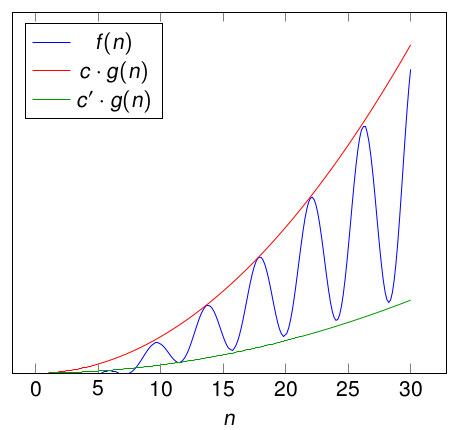
\includegraphics[width = \linewidth]{theta.png}}
Enfin, nous définissons l'ensemble des fonctions en $\Theta$ d'une autre fonction :
$$\begin{array}{c}
f(n) \in \Theta(n) \\
\strut \\
\iff \\
\strut \\
\exists c_1, c_2, n_0 >0 \;\; \mathrm{t.q} \;\; \boxed{c_1 \cdot g(n) \leq f(n) \leq c_2\cdot g(n)}\;\; \\ \forall n\geq n_0
\end{array}$$

\subsection{Classification des comportements asymptotiques}
En algorithmique, on cherche à évaluer le temps de calcul d'un algorithme et l'approcher en valeur asymptotique à une fonction "classique" parmi les suivantes, triées dans l'ordre croissant des tendances asymptotiques.
\begin{figure}[h]
\centering
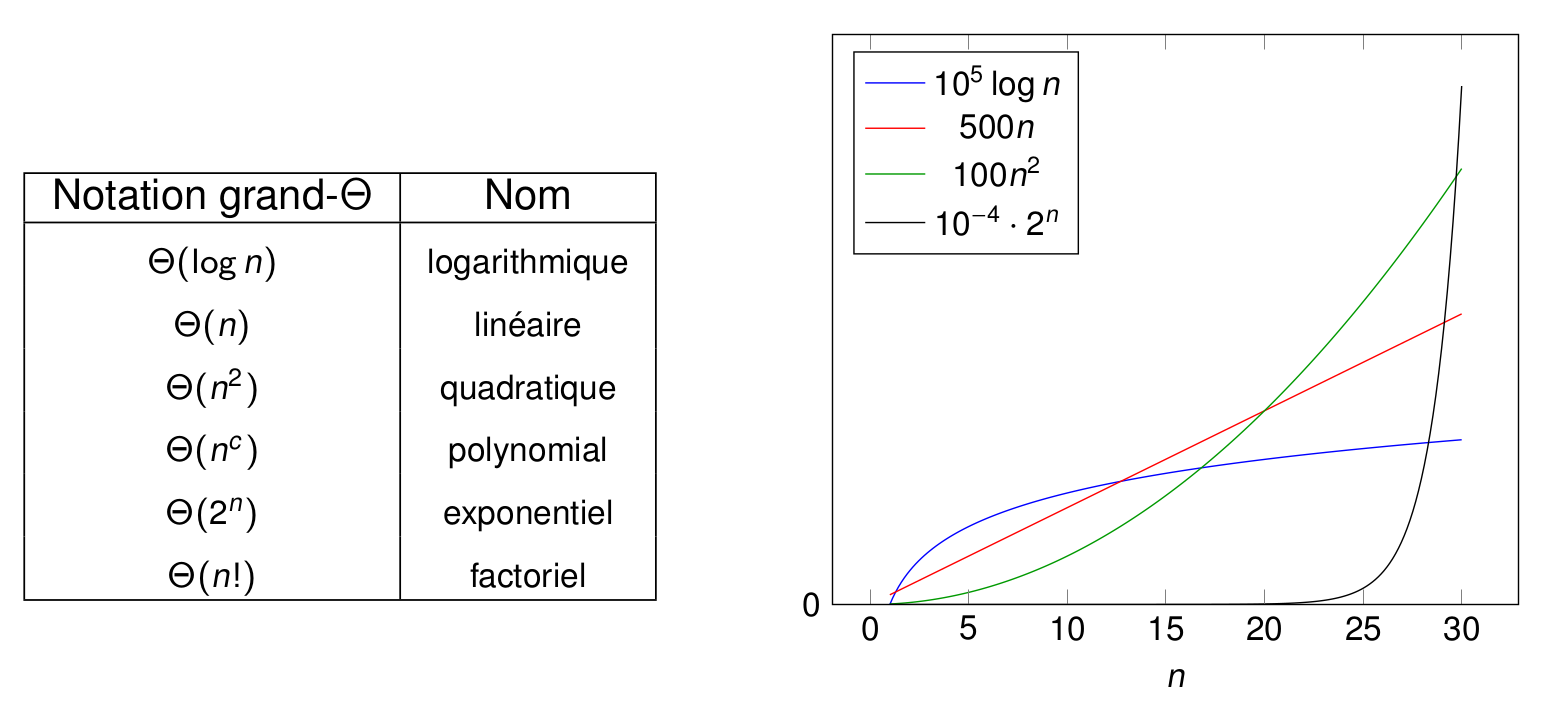
\includegraphics[width=0.8\linewidth]{croissances.png}
\caption{Tendances asymptotiques}
\end{figure}
\subsection{Complexité d'algorithme et de problème}
La \textbf{complexité d'un algorithme} est le comportement asymptotique de son temps de calcul $T(n)$ pour la \textbf{pire entrée}.\\

La \textbf{complexité d'un problème} est la complexité du meilleur algorithme pour ce problème. On précise "\textit{meilleur algorithme}" parce qu'un algorithme peut ne pas être optimal pour le problème qu'il résout.

\chapter{Problème de recherche de pic}
Le problème de la recherche de pic, d'abord à une dimension, puis à deux dimensions, consiste à chercher, dans un tableau, une valeur correspondant à un pic, c'est-à-dire plus grande que tous ses voisins contigus.
\section{Problème à 1D}
\subsection{Approche naïve}
L'apporche naïve consiste à parcourir toutes les valeurs une à une et pour chaque valeur, tester les deux voisins. C'est une approche qui marche mais qui est longue si chaque voisin de droite est plus grand que l'élément : dans le pire des cas, le temps est en $\Theta(n)$. La complexité de l'algorithme naïf est donc $n$.
\subsection{Algorithme \divc}
L'algorithme \divc, a.k.a "diviser pour régner", consiste à lire les deux valeurs en milieu de tableau : $a[\lfloor n/2\rfloor]$ et $a[\lfloor{n/2}\rfloor+1]$, et de les comparer. 

\begin{itemize}
\item Si $a[\lfloor{n/2}] > a[\lfloor{n/2}\rfloor-1]$, c'est qu'il y a un pic dans le tableau entre les indices $0$ et $\lfloor{n/2}\rfloor -1$. Il faut alors appliquer l'algorithme sur ce sous-tableau.

\item Si non, lire $a[\lfloor{n/2}\rfloor+1]$ et appliquer le même raisonnement.

\item Si non, c'est qu'il y a un pic à cet endroit-là.
\end{itemize} 
Dans le pire des cas, le pic ne se trouve jamais à l'endroit où on regarde, et on divise donc en 2 le tableau à chaque fois, jusqu') se réduire un tableau de taille minuscule : $n \rightarrow n/2^t$. Un pic est forcément atteint lorsque la taille du tableau vaut 1 ou 2, ce qui arrive lorsque 
$$n/2^t\approx 1 \iff t \approx \log n \quad \Longrightarrow \quad  \boxed{T(n) = \Theta\left(\log(n)\right)}$$

\section{Problème à 2D}
Dans un tableau bidimensionnel, il faut vérifier 4 voisins :
$$\begin{array}{rl}
a[i][j] \; \text{est un pic} \; \iff a[i][j] & \geq a[i-1][j] \\
& \geq a[i+1][j] \\
& \geq a[i][j+1] \\
& \geq a[i][j-1] \\
\end{array} $$
\subsection{Approche naïve -- greedy ascent}
L'approche naïve consiste à se déplacer dans le tableau dans la direction du voisin le plus grand. Encore une fois, ce n'est pas très économe parce que dans la pire des situations, dans un tableau de taille $n \times m$, on peut arriver à parcourir les $nm$ valeurs du tableau : $T(n) = \Theta(n^2)$
\subsection{\divc}
\wrap{10}{r}{0.4}{\vspace{-1cm}
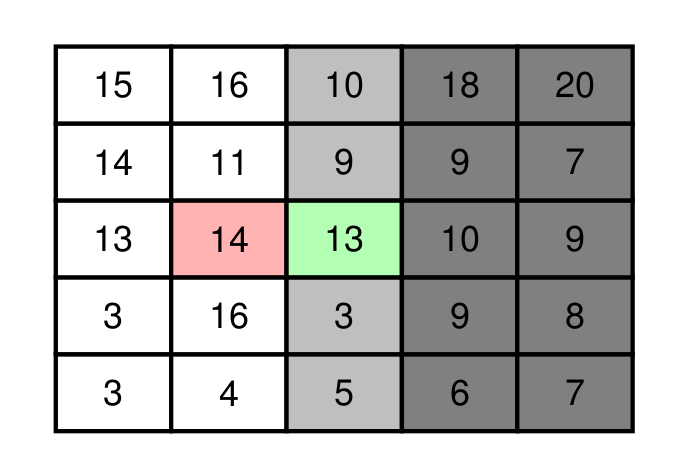
\includegraphics[width=0.8\linewidth]{pic_2D_div.png}
\caption{Application de l'algorithme \divc sur un tableau de taille $n\times m$}}
Encore cet algorithme ! Cette fois-ci, on commence par regarder la colonne du milieu en cherchant le maximum global de la colonne (temps en $\Theta(n)$). On compare ce maximum à ses voisins de gauche et de droite et on applique l'algorithme sur le tableau de gauche ou de droite selon quel voisin est plus grand que $a[i][\lfloor m/2 \rfloor]$ (le maximum de la colonne du milieu). \\

L'analyse de la complexité de cet algorithme est simple :
\begin{enumerate}
\item Trouver un maximum global : $\Theta(n)$
\item Appliquer l'algorithme sur un tableau $n\times (m/2)$
\end{enumerate}
$$\begin{array}{rl}
\text{Cas de base} &: \quad  T(n,1) = \Theta(n) = C \\
T(n,m) &= C + T(n, m/2)
\end{array}
$$
Cela veut dire qu'à chaque étape, on ajoute $C+T(n, m/2)$ jusqu'à arriver à $m=2$ où $m/2 = 1$ et on revient au cas de base. La récurrence est donc facilement résolue :

$$\boxed{T(n,m) = \Theta\left(n\cdot \log m\right)}$$

Nous voyons donc qu'un algorithme \divc permet d'améliorer grandement la complexité par rapport à une approche "naïve".

\section{Réflexion algorithmique}
\begin{enumerate}
\item Analyser la définition du problème : existence de solution ? cas particuliers ?
\item Considérer tous les cas possibles
\item Analyser les propriétés de l'alrogithme conçu : se termine-t-il ? est-il toujours correct ?
\item Analyser la complexité : le pire cas
\item Se demander si l'on peut faire mieux
\end{enumerate}

\chapter{Algorithmes de tri}
\section{Motivation}
Il y a un besoin intrinsèque d'avoir des données triées. Que ça soit pour avoir un \textbf{ordre} dans les données (dictionnaire, annuaire), ou pour résoudre certains problèmes plus rapidement, ou pour des applications plus technologiques comme la compression de données et le rendu d'effets graphiques. \\

Pour un problème de tri, nous avons pour entrée un tableau $a$ de taille $n$ à ordonner. La sortie serait une permutation de tableau de sorte que 
$$a'[0]\leq a'[1]\leq a'[2]\leq\cdots \leq a'[n-1]$$
\section{Tri par insertion}
\subsection{Approche idiote}
Une première idée, et sans doute la pire de l'histoire du tri, est de parcourir le tableau, valeur par valeur, et de placer chaque élément dans un nouveau tableau de sorte que ce-dernier soit trié. Non seulement il faut parcourir tout le tableau, mais en plus de ça le tri n'est \textbf{pas en place} (on travaille sur une copie du tableau), mais aussi : si le tableau est trié initialement dans l'ordre décroissant, il faudra décaler les $n-1$ éléments du tableau créé pour placer l'élément $a[n-1]$. \\


\subsubsection{Meilleur cas}
Notons que dans le meilleur cas, celui où le tableau est déjà trié, le coût de traitement de l'élément d'indice $i$, que nous allons noter $C_i$, est indépendant de $i$ : il ne faut rien décaler, juste ajouter en fin de tableau.

\subsubsection{Pire cas}
Soit le pire des cas, celui bien précis où le tableau est initialement dans l'ordre inverse. À l'insertion de l'élément d'indice $i$, il faudra effectuer $i$ \textbf{permutations}. En effet, vu que le tableau est dans l'ordre décroissant, à chaque fois qu'on va vouloir mettre une valeur dans le nouveau tableau copié, celle-ci sera inférieure à toutes les valeurs déjà dans le tableau : donc il faudra bouger chacune vers la droite, ce qui prend un temps constant par élément, mais il faudra le faire $n_i$ fois pour l'élément d'indice $n_i$ ! Le temps de calcul vient alors, en notant $C_i$ le coût de traitement de l'élément d'indice $i$ :
$$C_i = c \cdot i \; ;$$
et pour l'ensemble des $n$ éléments à trier :
$$T(n) = \sum_{i=1} ^{n-1} C_i = c\cdot \dfrac{n(n-1)}{2} = \Theta(n^2)$$
\subsection{Approche par recherche dichotomique}
Une deuxième approche, mieux que la première, serait de regarder à chaque élément $i$, où est le meilleur endroit pour insérer : cela se fait en faisant une recherche dichotomique sur le nouveau tableau avec les $i-1$ éléments déjà dedans. Il faudra alors, à chaque insertion (il y en a $n$), effectuer $\log(i)$ comparaisons si nous insérons l'élément $i$. En revanche il faudra toujours effectuer le même nombre de permutations ! Le calcul suivant vient alors :
\subsubsection{Comparaisons}
On réduit le nombre total de comparaisons : 
$$T'(n) = \sum_{i=1} ^{n-1} \log(i) = \log\left(\prod_{i=1}^{n-1} i\right) = \log\left((n-1)!\right) = \Theta\left(n\cdot \log(n)\right)$$
\subsubsection{Permutations}
On ne change pas le nombre de permutations !
$$T(n) = \sum_{i=1} ^{n-1} C_i = c\cdot \dfrac{n(n-1)}{2} = \Theta(n^2)$$
On l'aura compris, le but ultime est de réduire également le nombre de permutations. En tout cas pour le tri par insertion, quoique l'on fasse, on effectue $n$ permutations et on revient à un temps en  $n^2$.
\bb{Coût du tri par insertion : $T(n) = \Theta(n^2)$}
\section{Le tri par fusion -- approche \divc}
\subsection{Principe}
Le problème du tri peut également être abordé par une approche \divc . L'objectif serait d'appliquer récursivement le même algorithme sur une sous-partie du tableau et de recombiner tous les morceaux à la fin.
\subsection{Canevas général d'un algotithme \divc}
En toute généralité, un algorithme \divc s'écrit de la manière qui suit :
\begin{figure}[h]
\centering
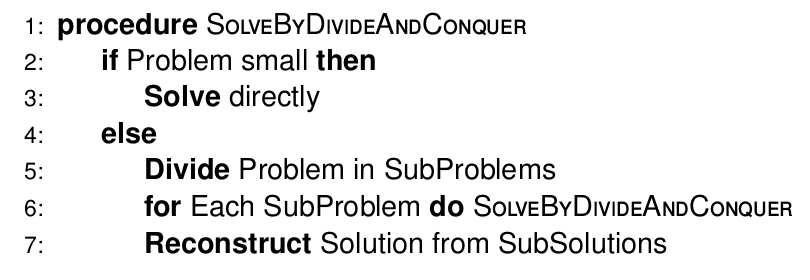
\includegraphics[width=0.6\linewidth]{div_pseudoc.png}
\caption{Canevas général d'un algorithme \divc}
\end{figure}
\begin{figure}[h]
\centering
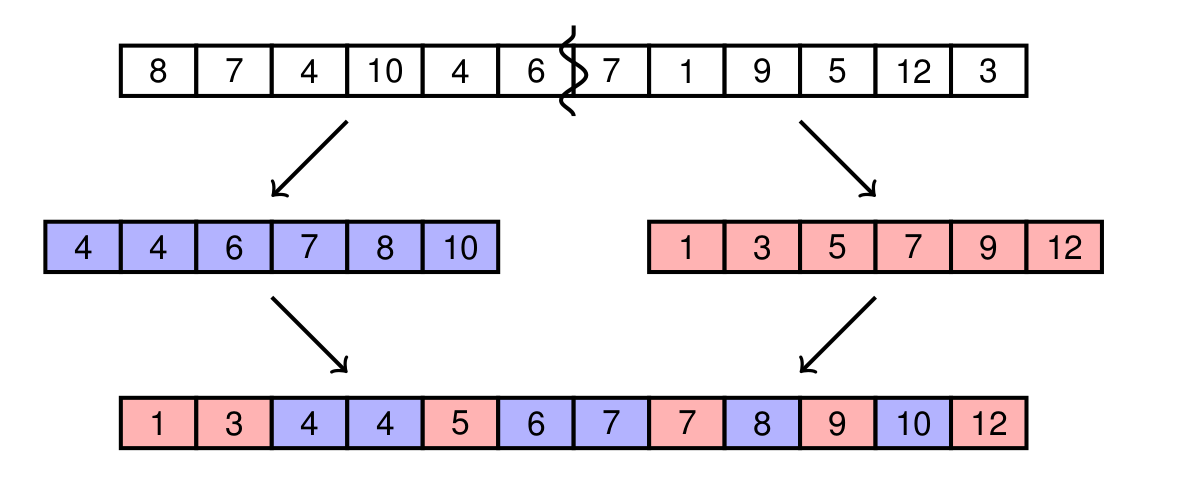
\includegraphics[width=0.6\linewidth]{tri_fus_ill.png}
\caption{Illustration du tri par fusion où les pseudo-codes sont donnés par les figures \ref{fig:tri_fus_pseudoc} et \ref{fig:tri_fus_merge}.}
\label{fig:tri_fus_ill}
\end{figure}
\subsection{Application au problème de tri}
\subsubsection{Pseudo-code}
\wrap{8}{r}{0.4}{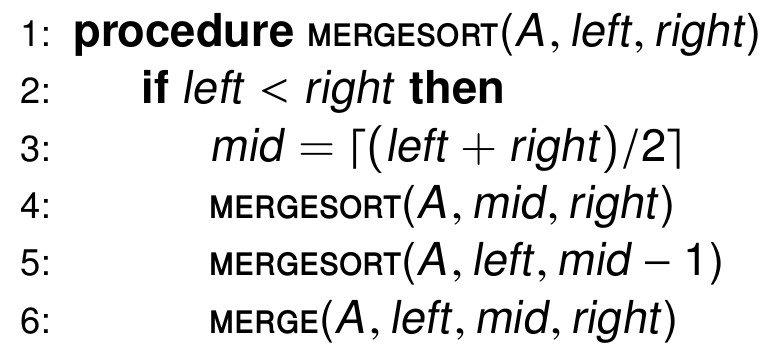
\includegraphics[width=0.9\linewidth]{tri_fus_pseudoc.png}
\caption{Pseudo-code du tri par fusion}
\label{fig:tri_fus_pseudoc}}
Pour l'appliquer \textbf{en place}, il faut travailler sur le même tableau et donc le trier entre certains indices, par exemple : trier le tableau entre les indices $a$ et $b$, entre $b$ et $c$, et puis combiner les deux sous-tableaux. On a donc naturellement le pseudo-code ci-contre, où il faut encore définir la procedure \code{merge} que nous voyons apparaître : comment fusionner deux sous-tableaux ?
\subsubsection{Fusion de deux sous-tableaux triés}
Vu que les deux sous-tableaux sont déjà triés, il sera facile de les fusionner en un tableau trié. Si un tableau $A$ est donné en entrée et étant constitué de deux tels sous-tableaux, la première chose à faire sera de créer deux copies des sous-tableaux, pour appliquer les modifications sur $A$ lui-même. Comme avant, pour que le tri se fasse entièrement en place, on va considérer en entrée la liste d'arguments : $A$, indice de gauche \code{left}, indice de droite \code{right} et indice de milieu \code{mid}. Le début du tableau de gauche serait alors $n_L =$\code{mid} - \code{left}, celui du droit serait $n_R = $ \code{right}-\code{mid}+1. \\

Ensuite, il suffira de comparer les éléments du tableau de gauche aux éléments du tableau de droite et de placer dans $A$ le plus petit d'entre les deux. Si on arrive à comparer deux "infinis", c'est-à-dire des éléments qu'on a placé expressément à la fin des deux sous-tableaux pour indiquer qu'on s'y est baladé jusqu'à la fin, c'est qu'on a terminé le tri.

\begin{figure}[h]
\centering
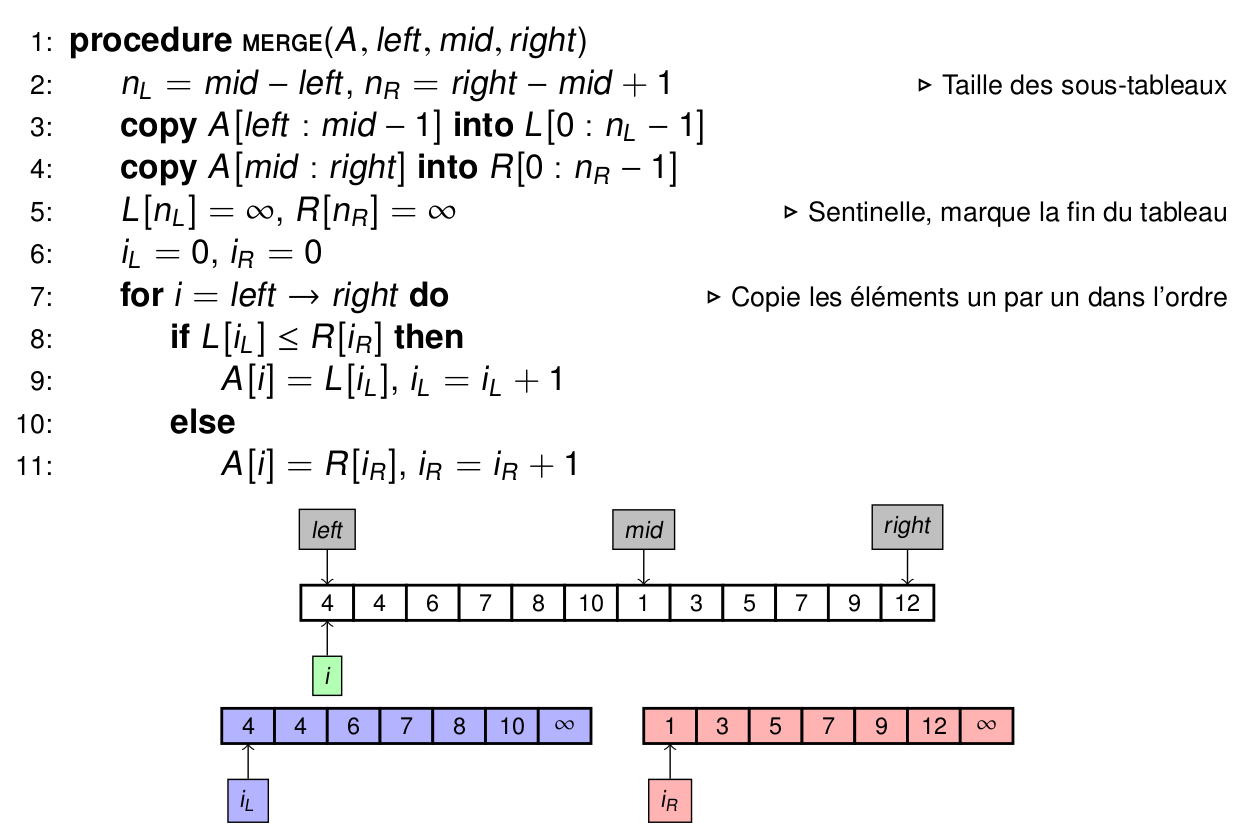
\includegraphics[width=0.9\linewidth]{tri_fus_merge.png}
\caption{Pseudo-code de la fusion de deux sous-tableaux triés, utile pour le tri par fusion.}
\label{fig:tri_fus_merge}
\end{figure}
\subsubsection{Complexité de \code{merge}}
Faire un \code{merge} nécessite deux choses : 
\begin{itemize}
\item faire une copie de chaque sous-tableau : $\Theta(n_L + n_R) = \Theta(n)$, 
\item faire des affectations simples (indices $n_L$, $n_R$, ...) : $\Theta(c_2)$
\item faire une boucle entre \code{left} et \code{right} soit $n$ itérations. Pendant chaque itération, des opérations qui prennent un temps constant sont faites $\Rightarrow \Theta(c_1 n)$.
\end{itemize}
Le coût total d'un \code{merge} est donc $$T(n) = c_1 \cdot n + c_2 \; .$$
\subsubsection{Complexité de \code{mergesort}}
La complexité du tri par fusion s'obtient en résolvant une récurrence et ceci est fait en détails dans le TP. Dans les grandes lignes, on fait un tri par fusion en  :
\begin{itemize}
\item séparant le tableau en deux sous-tableaux : affectation d'indices, temps constant $c_4$,
\item en appliquant l'algorithme sur le tableau de taille $\lfloor n/2\rfloor$ : $T(\lfloor n/2\rfloor)$
\item en appliquant l'algorithme sur le tableau de taille $\lceil n/2\rceil$ : $T(\lceil n/2\rceil)$
\item effectuer un \code{merge} : $c_1 \cdot n + c_2$
\end{itemize} 
Le total est donc :
$$T(n) = T(\lfloor n/2\rfloor) + T(\lceil n/2\rceil) + c_1 \cdot n + \bleu{c_2 + c_4}$$
La récurrence est donc à résoudre avec le cas de base $T(1) = c_3$. Les feuilles de l'arbre de récurrence sont donc de valeur $c_3$ (que nous allons noter $c$). Pour \textbf{simplifier}, on ignore les \bleu{termes constants négligeables}, on suppose que $n$ est une puissance de 2 et on pose $c = \max(c_1, c_3)$ :

$$\boxed{T(n) = 2\cdot T(n/2) + c\cdot n}$$
En résolvant l'arbre de récurrence, on obtient : $c\cdot n$ pour le total de chaque étage, et une hauteur de $\log n$, donc en comptant la racine de l'arbre :

\bb{Coût du tri par fusion : $T(n) = \Theta(n\cdot \log n)$}
\section{Conclusion}
L'approche \divc apporte encore un gain asymptotique par rapport au tri par insertion. Le problème ici est que le tri par fusion n'est \textbf{pas en place}, il requiert un espace auxiliaire en mémoire de taille $\Theta(n)$. \\

Cependant, le facteur multiplicatif devant le $\log(n)$ n'est pas rassurant vu qu'il s'agit d'un $n$. Il faudra mieux alors \textbf{appliquer le tri par insertion pour les tableaux de petite taille}, et le tri par fusion pour les tableaux de grande taille.
\section{Tri par tas}
Le tri par tas est une méthode de tri qui a été introduite en même temps que la structure de données qu'on appelle "\textbf{tas}", présentée dans le chapitre suivant. De n'importe quel tableau il est possible de former un \textbf{tas}, en place (sans devoir réattribuer de la place en mémoire) et sans surcoût lié à la taille du tableau car la création d'un tas de taille $n$ est en $\Theta(n)$. La particularité d'un tas est que le maximum se trouve toujours en première position : on peut le mettre en fin de tableau avec une méthode en $\Theta(\log (n))$. Le tri par tas a un coût en $\Theta(n\cdot\log (n))$ et est en place.
\section{Quicksort}
Le \textit{quicksort} consiste en une méthode de type \divc "alternative" : on réordonne le tableau \textbf{autour d'un élément}, le pivot, de sorte que les éléments à gauche du pivot lui soient inférieurs et que les éléments à droite lui soient supérieurs.
$$A[0:n-1] \longrightarrow A[q] \quad \text{t.q} \quad \left\{\begin{array}{ll}
\forall i \in [0,q-1] : &A[i] < A[q] \\
\forall i \in [q+1,n-1] : &A[i] > A[q] \\
\end{array}\right.$$
\subsection{Partitionnement}
\subsubsection{Principe}
Le tri rapide consiste à trier des sous tableaux avec un appel récursif à chaque fois. Chaque appel récursif est de la forme \pseudo{Quicksort(A, Left, Right)}. À chaque appel, on effectue une \textbf{partition du tableau} : c'est une méthode qui prend comme pivot l'élément à droite du tableau et qui 
\begin{itemize}
\item place tous les éléments inférieurs à \pseudo{A[Right]} à gauche dans le tableau,
\item place tous les éléments supérieurs à \pseudo{A[Right]} à droite dans le tableau,
\item place le pivot à la séparation entre les deux zones.
\end{itemize}
Cela se fait en déterminant la valeur de \pseudo{A[Right]}, en comparant chaque élément, de \pseudo{A[Left]} à \pseudo{A[Right-1]}, et en définissant un indice $i$ correspondant à la frontière entre les zones "plus petit" et "plus grand". $i$ est donc incrémenté de $1$ à chaque fois qu'une valeur plus \textbf{petite} que \pseudo{A[Right]} est parcourue. Alors, cette valeur est échangée avec l'élément $i+1$ et $i$ s'incrémente de 1.
\begin{figure}[h]
\centering
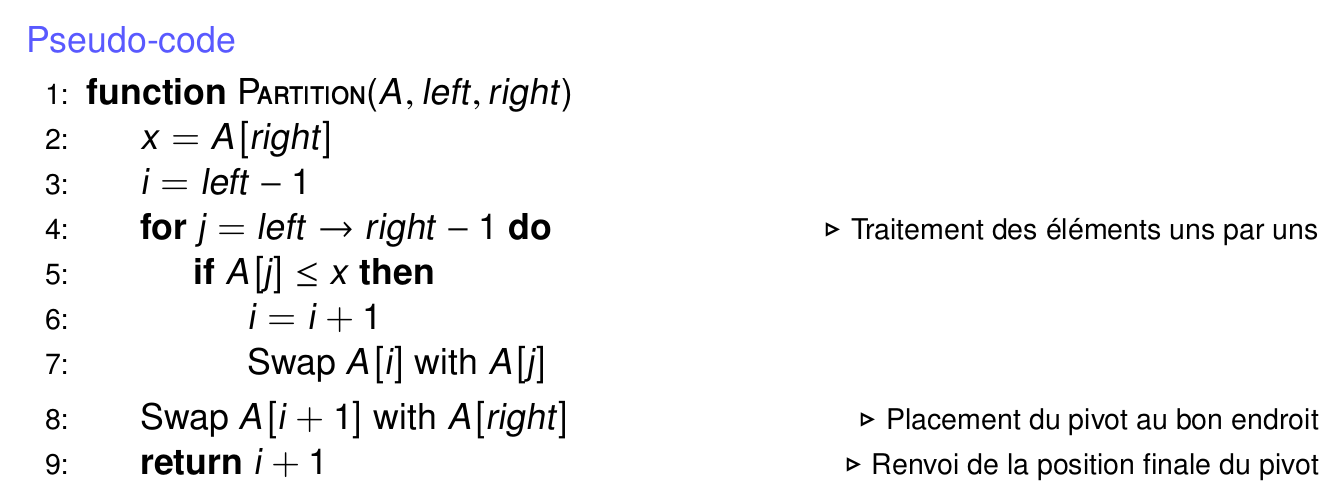
\includegraphics[width=0.8\linewidth]{quicksort_part_pseudoc} \\
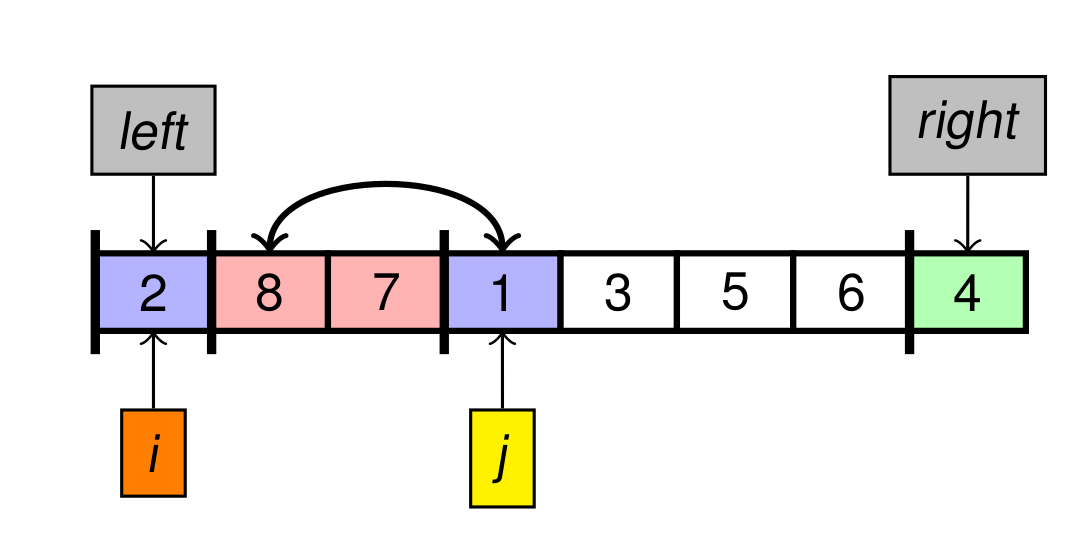
\includegraphics[width = 0.3\linewidth]{quicksort_part1} 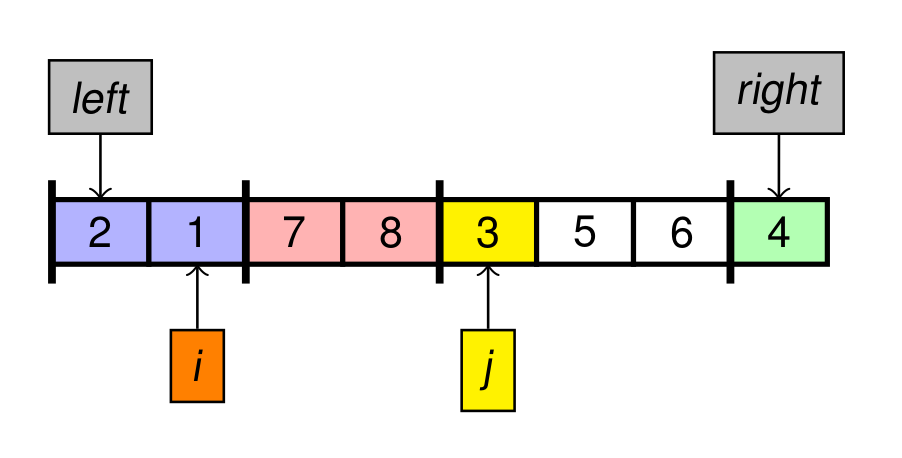
\includegraphics[width = 0.3\linewidth]{quicksort_part2} 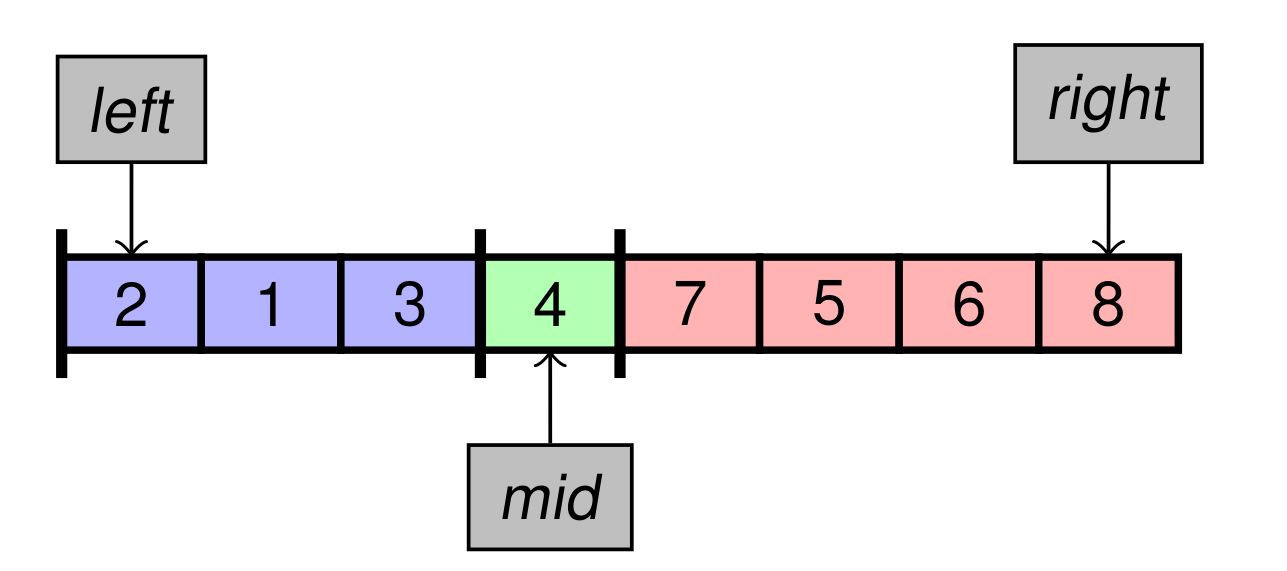
\includegraphics[width = 0.3\linewidth]{quicksort_part3}
\caption{Pseudo-code et illustration de la partition d'un tableau sur base d'un indice de gauche et un indice de droite. Valeur de retour : la position du pivot après partition.}
\label{fig:quicksort_part}
\end{figure}
\subsubsection{Coût du partitionnement}
Pour le \textbf{pire partitionnement}, qui est le premier, le programme parcourt tout le tableau. A chaque fois, il effectue des opérations constantes comme une comparaison, etc. Et en prime il y a quelques assignations dans le programme. Le cout pour partitionner le tableau est donc en $\Theta(n)$
$$T(n) = T(c_1\cdot n + c_2) = \Theta(n)$$

\subsection{L'algorithme du quicksort}
L'algorithme du quicksort consiste à commencer par partitionner le tableau avec comme indices \pseudo{Left} et \pseudo{Right} : ceci retournera la position du \textbf{pivot} (initialement l'argument passé dans \pseudo{Right} de la fonction) une fois que les échanges de la figure \ref{fig:quicksort_part} auront été effectués. Après ça, un quicksort sera appliqué sur le tableau de gauche puis sur le tableau de droite, sans préférence particulière.
\begin{figure}[h]
\centering
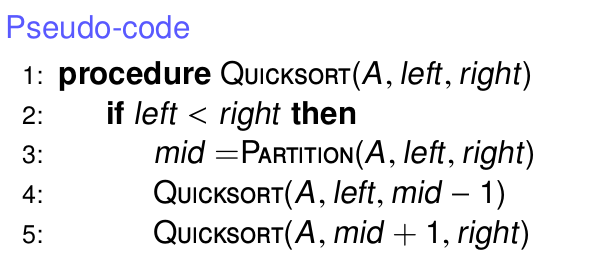
\includegraphics[scale=0.4]{quicksort_pseudoc}
\caption{Pseudo-code de l'algorithme de tri rapide.}
\label{fig:quicksort_pseudo}
\end{figure}

\subsection{Complexité du tri rapide}
A chaque appel de \pseudo{Quicksort}, un appel à \pseudo{Partition} est fait, un algorithme qui prend un temps $c_1\cdot n + c_2$, et deux appels sont faits à \pseudo{Quicksort}. Nous avons ainsi por la complexité totale :
$$\begin{array}{lll}
T(n) =& T_1(n) \qquad=  &c_1\cdot n + c_2 \\
	&+ T_2(n) 	&+ T(n_{\text{left}}) \\
	&+ T_3(n)	&+ T(n_{\text{right}})
\end{array}$$
où $n_{\text{left}} = \pseudo{mid} - \pseudo{left}$ et $n_{\text{right}} = \pseudo{right} - \pseudo{mid}$, et \pseudo{mid} est justement déterminé par l'appel à \pseudo{Partition}. Autrement dit, le temps mis par l'algorithme dépend de la position du pivot : il dépend de l'instance du problème. 
\begin{figure}
\centering
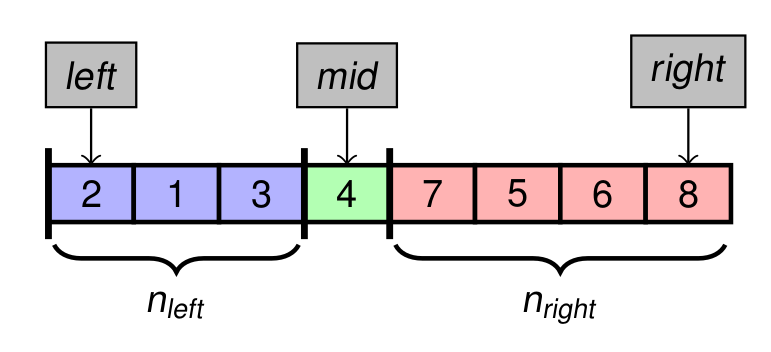
\includegraphics[scale=0.4]{quicksort_complexite_nleftright}
\caption{Signification des variables $n_{\text{left}}$ et $n_{\text{right}}$ après un appel à \pseudo{Partition} qui renvoie la valeur de \pseudo{mid}.}
\label{fig:quicksort_complexite_nleftright}
\end{figure}

\subsubsection{Complexité -- meilleur cas}
Etudions la complexité dans le meilleur des cas : c'est celui où le partitionnement est \textbf{parfaitement équilibré} $\Rightarrow n_{\text{left}} \approx n_{\text{right}} \approx n/2$. Alors, le temps mis par l'algorithme est donné par :
$$T(n) = 2\cdot T(n/2) + c\cdot n = \Theta(n\cdot \log(n))$$
après résolution de l'arbre de récurrence.

\subsubsection{Complexité -- pire cas}
Le pire cas correspond à la situation où le partionnement est \textbf{complètement déséquilibré}, et ce, à \textbf{chaque étape du tri} : $n_{\text{left}} = n-1$ et $n_{\text{right}} = 0$ comme on peut l'imaginer sur la figure \ref{fig:quicksort_complexite_nleftright}. Dans ce genre de situations, la récurrence s'écrit :
$$T(n) = T(n-1) + c\cdot n$$
et l'arbre de récurrence est un arbre avec des branches d'un seul côté, à chaque noeud. La taille de l'arbre étant de $n$, on peut trouver facilement le coût de l'algorithme, car chaque étage est $n$ décrémenté de $1$. Plus précisément, pour le calcul de la complexité, on part du cas de base (le bas de l'arbre) $T(1)=c$, et on remonte chaque branche en incrémentant la hauteur de $1$, et en ajoutant un $c\cdot i$ jusqu'à atteindre $c\cdot n$. Ainsi :
$$T(n) = \sum_{i=1} ^n c\cdot i = c \cdot \dfrac{n(n+1)}{2} = \Theta(n^2)$$
Nous observons alors que pour un partionnement très déséquilibré, ce qui correspond par ailleurs à un tableau déjà trié (!), la complexité est en $\Theta(n^2)$. Pour le tri par insertion, le tri d'un tableau déjà trié prend un temps $\Theta(n)$... Que devons-nous conclure de ça ? Venons-nous d'apprendre une méthode de tri inutile ? \\

Nous allons montrer dans la section suivante qu'en \textbf{moyenne}, la complexité de l'algorithme \pseudo{Quicksort} est en $\Theta(n\cdot\log(n))$.
\subsubsection{Complexité -- cas moyen}
Si nous supposons que nous avons un partitionnement \textit{légèrement déséquilibré}, du style $n_r = n/10$ et $n_l = 9n/10$, alors le raisonnement de la figure \ref{fig:quicksort_complexite_moyen} mène à une complexité en $O(n\cdot \log(n))$.  
\begin{figure}[h]
\centering
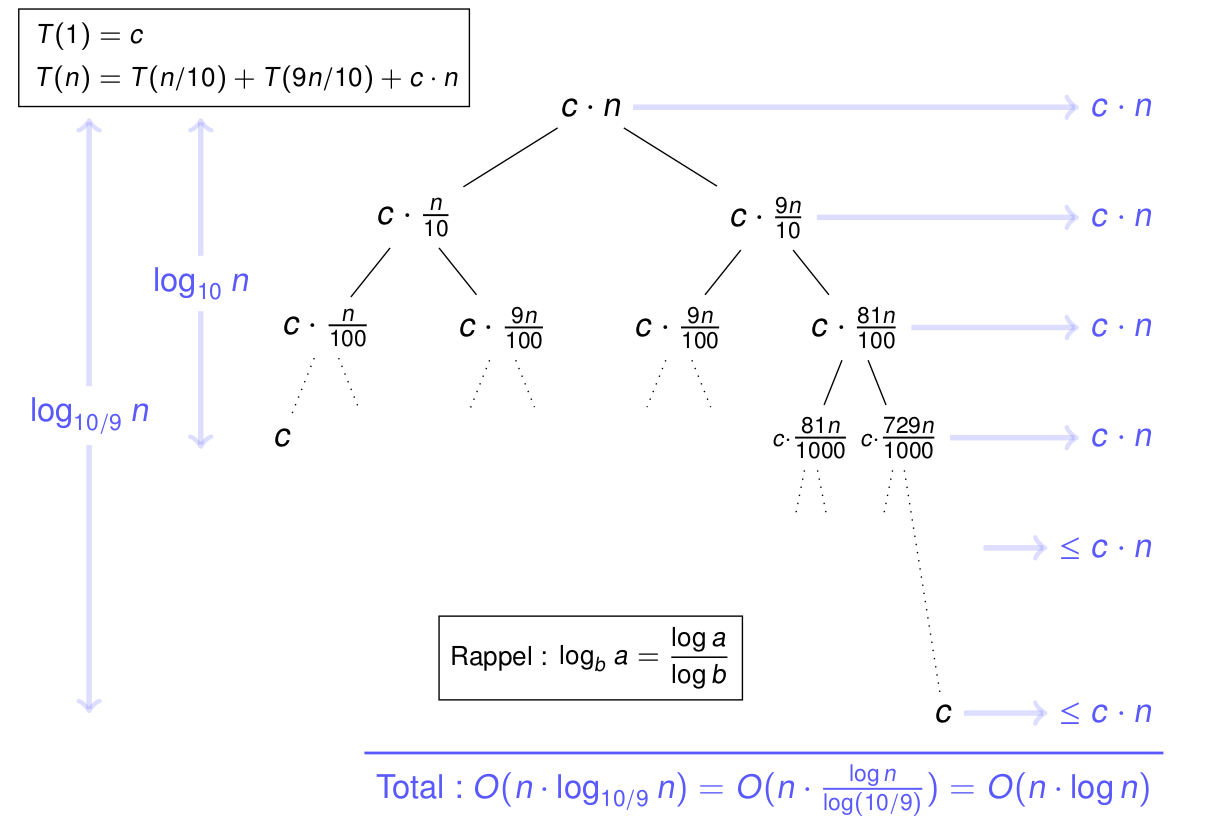
\includegraphics[width=0.7\textwidth]{quicksort_complexite_moyen}
\caption{Arbre de récurrence de l'algorithme \pseudo{Quicksort} si le partitionnement est tel que $n_r = n/10$ et $n_l = 9n/10$ \textbf{à chaque étape}.}
\label{fig:quicksort_complexite_moyen}
\end{figure}
Nous constatons en effet que nous avons des étages à $c\cdot n$ qui finissent par se terminer à une hauteur de $\log_{10}(n)$ tandis que d'autres branches continuent jusqu'à une hauteur $\log_{10/9} (n)$ : il y a moins d'un total de $c\cdot n$ à ce dernier étage. Nous pouvons donc borner supérieurement à l'aide d'un $O$ le temps mis par l'algorithme :
$$T(n) = O(n\log_{10/9} (n)) = O(n\cdot \log(n)) \; .$$

Si nous voulons nous \textbf{assurer} d'avoir un partitionnement meilleur que $(9/10, 1/10)$, il faut que le pivot soit soit plus grand soit plus petit que $10\%$ des éléments : cela arrivera dans $80\%$ des cas. \\

\subsection{Tri rapide avec aléatoire}
Comme on vient de le voir, il n'est pas toujours intéressant d'appliquer le tri rapide quand on prend comme pivot l'élément le plus à droite du tableau. Pour assurer la légitimité du tri rapide, nous allons introduire le fait qu'une \textbf{analyse probabiliste rigoureuse non-vue au cours} permet d'assurer que \textit{si le pivot est choisi au hasard parmi tous les éléments du tableau, alors en moyenne, la complexité de l'agorithme de tri rapide est en $\Theta\left(n\cdot\log(n)\right)$, et ce quel que soit l'ordre initial du tableau}.
\begin{figure}
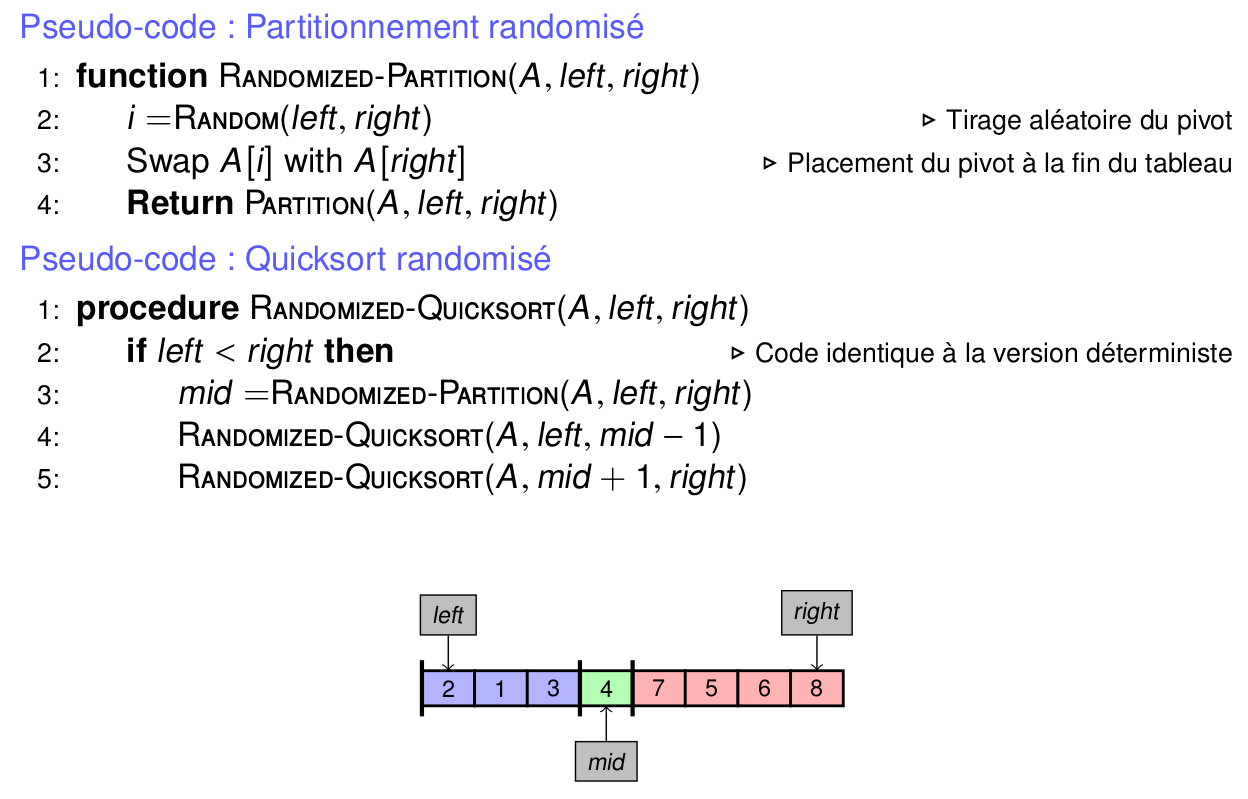
\includegraphics[width=0.8\linewidth]{quicksort_randomized}
\caption{Pseudo-code de l'algorithme de tri rapide avec partitionnement aléatoire.}
\label{fig:quicksort_randomized}
\end{figure}

\section{Tris par comparaison -- borne inférieure pour le tri}
Faisons un récapitulatif des algorithmes de tri vus jusqu'à présent :
\begin{table}[h]
\begin{center}
\begin{tabular}{|c|c|c|c|}
\hline
 				&	$\Theta(n^2)$ & $\Theta(n)$ & $\Theta(n\cdot\log(n))$ \\
 				\hline
 Pire cas 		& 	Tri par insertion & & \begin{tabular}{c} Mergesort \\
 Heapsort
 \end{tabular} \\ \hline
 Meilleur cas 	&	& Tri par insertion & \\ \hline
 En moyenne		& & & Quicksort \\ \hline
\end{tabular}
\end{center}
\end{table}
\subsection{Peut-on encore faire mieux ?}
C'est ambitieux de vouloir un temps plus court que du $\Theta(n\cdot\log(n))$ : on a déjà vu 4 algorithmes et 3 de ceux-ci rivalisent très clairement mais s'alignent selon ce temps. 
\subsection{Arbres de décision}
En réalité, on peut montrer que \textbf{si le tri est un tri par comparaison}, c'est-à-dire si l'ordre final est déterminé uniquement par comparaisons antre éléments, alors un algorithme de tri en $\Theta(n\cdot\log(n))$ est optimal. C'est en dressant l'arbre de décision du tri que l'on détermine le nombre de comparaisons à effectuer au minimum pour trier les éléments d'un tableau qu'on se rend compte que cette borne inférieure est $n\cdot \log(n)$. \\

Dans cet arbre, nous observerons les éléments suivants :
\begin{itemize}
\item $h$ la hauteur du tableau : la hauteur de la plus basse feuille. C'est aussi le nombre \textbf{maximum de comparaisons} à effectuer pour trier un tableau.
\item $l \leq 2^h$ le nombre de feuilles, car l'arbre est un arbre \textbf{binaire}
\item $n! \leq l$ le nombre d'ordres finaux possibles pour $n$ éléments : $n! = l$ pour les algorithmes déterministes.
\end{itemize}
\begin{figure}[h]
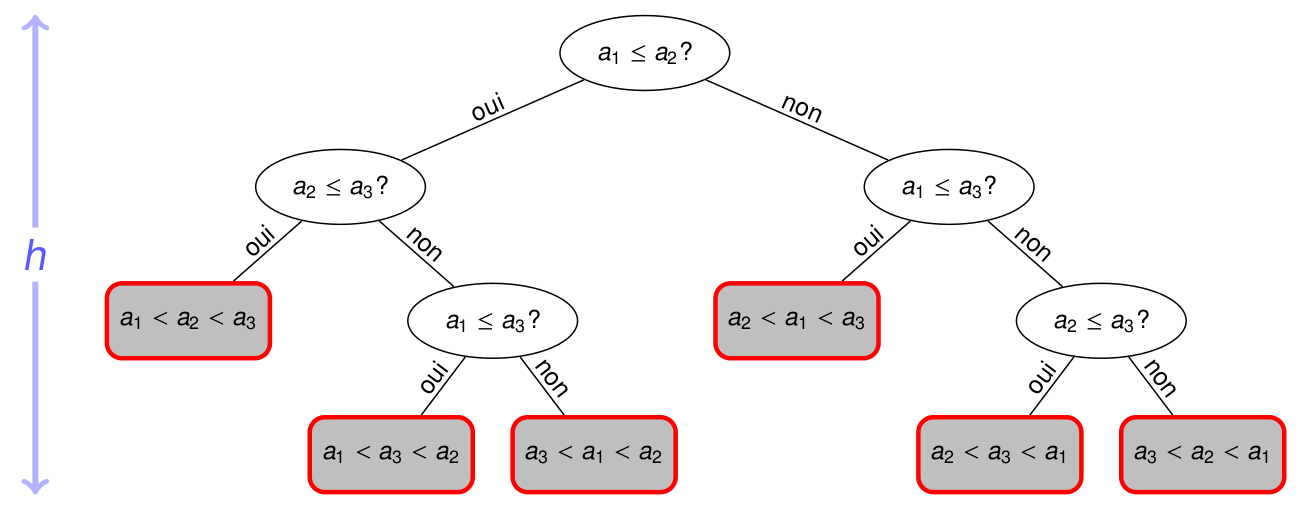
\includegraphics[width=0.8\linewidth]{tri_comparaison_arbre.png}
\caption{Arbre de décision lors du tri d'un tableau de 3 éléments. Nombre d'ordres finaux possibles : $n!$}
\end{figure}
A la lumière des notions introduites, nous pouvons écrire sereinement $$h \geq \log(n!) \; ,$$ et étant donné le théorème suivant très important pour le raisonnement, nous pourrons conclure sur une borne inférieure pour le tri par comparaison.

\bb{Théorème : $\log(n!) = \Theta(n\cdot\log(n))$}
Ainsi, $$h \geq \log(n!) = \Theta(n\cdot\log(n))$$ $\Rightarrow$ tout algorithme requiert donc $\Omega(n\cdot\log(n))$ comparaisons pour faire un tri par comparaison.
\subsection{Conclusion}
Tous les algorithmes de tri doivent faire au moins $\Omega(n\cdot\log(n))$ comparaisons. La complexité est donc en $\Omega(n\cdot\log(n))$, ce qui consitue une \textbf{borne inférieure}. Or pour certains algorithmes, comme \pseudo{Mergesort} ou \pseudo{Heapsort}, la complexité est en $\Theta(n\cdot\log(n))$ dans le pire des cas : ils sont donc \textbf{optimaux pour le modèle de tri par comparaison}.

\section{Tri linéaire}
Le tri linéaire n'est pas un tri par comparaison. Comme son nom l'entend, son but est de trier un tableau en un temps linéaire.
\subsection{Tri par comptage (counting sort)}
Très brièvement, le but est d'ici trier un tableau en comptant les valeurs en doublon dans le tableau, et ensuite de créer un tableau trié dans lequel on copie les éléments du premier tableau. Attention : ici on suppose qu'un élément du tableau est un objet et pas juste un entier, il faut donc s'assurer de copier l'objet lui-même et pas juste la valeur de la clé ! \\

Nous allons appliquer cet algorithme sur un tableau de $n$ objets où les clés prennent $k$ valeurs différentes.

\subsection{Pseudo-code du tri par comptage}
Le pseudo code consiste en 4 boucles :
\begin{enumerate}
\item La première boucle itère sur toutes les $k$ valeurs que peuvent prendre les clés : on initie le tableau de comptage $C$ $\Rightarrow$ coût en $\Theta(k)$.
\item La deuxième boucle est une itération sur tous les éléments du tableau, et on incrémente $C[A[j]]$ pour tous les $j$ allant de $0$ jusqu'à $n-1$ : c'est un coût en $\Theta(n)$.
\item La troisième boucle est assez bizarre : elle fait contenir dans $C[i]$ le nombre d'éléments dont la clé est inférieure à $i$. Ca a l'air bizarre mais c'est utile pour la boucle d'après $\Rightarrow$ coût en $\Theta(k)$.
\item Enfin, la dernière boucle place $A[j]$ dans le tableau trié : $B[C[A[j]] - 1] = A[j]$, et puis décrémente $C[A[j]]$ de $1$ pour "mettre à jour la place du prochain élément" $\Rightarrow$ coût en $\Theta(n )$.
\end{enumerate}

\begin{figure}[h]
\centering
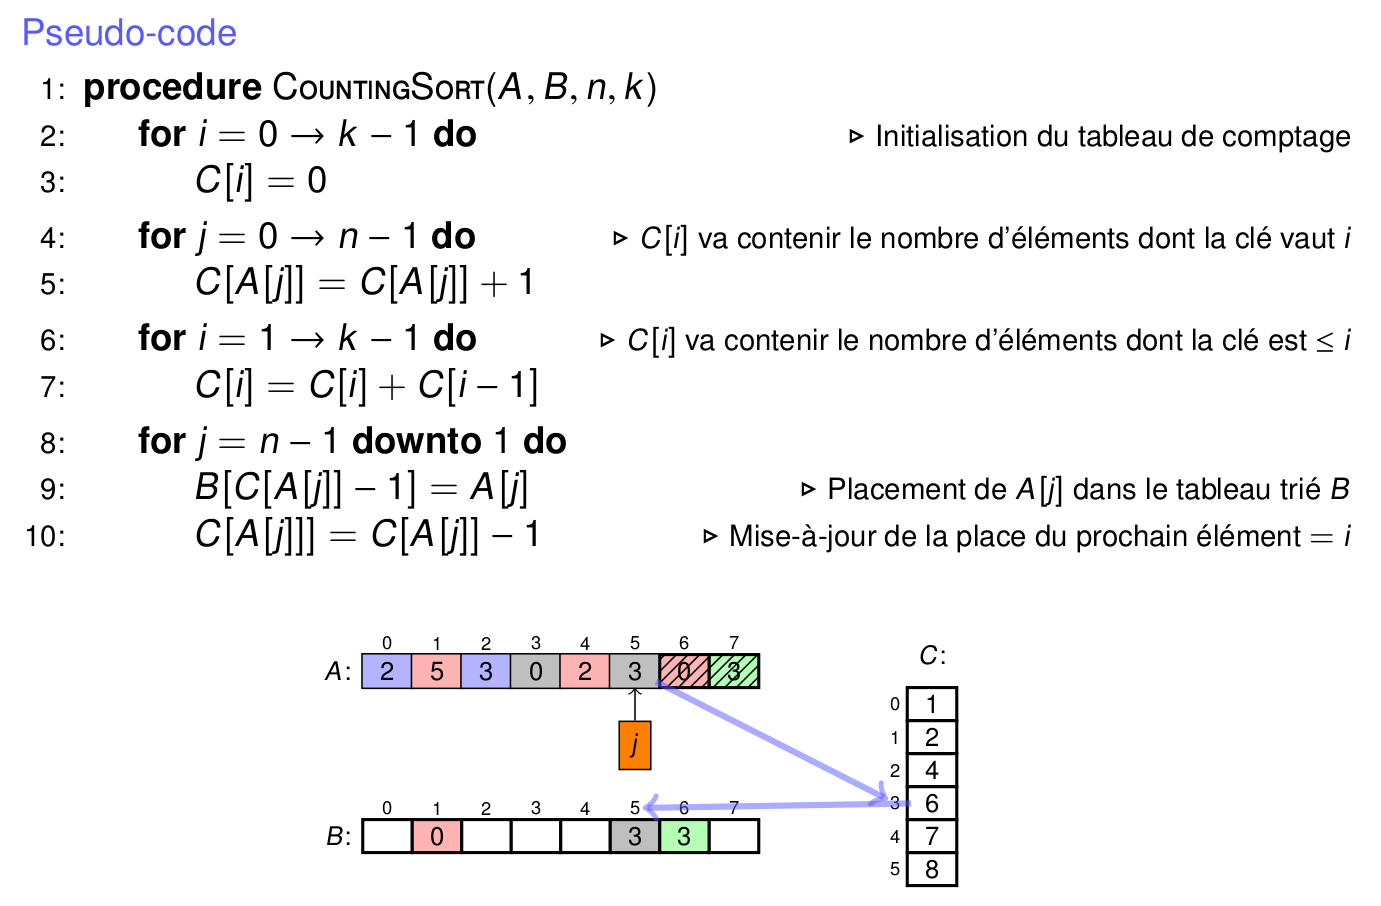
\includegraphics[width=0.8\linewidth]{tri_lineaire.png}
\caption{Pseudo-code du tri linéaire.}
\label{fig:tri_lineaire.png}
\end{figure}

Le coût total est en $\Theta(n+k)$, ce qui revient à $\Theta(n)$ si $k = O(n)$. C'est donc possible d'avoir un coût plus faible que $\Theta(n\cdot\log(n))$ car les informations sont obtenues autrement que par comparaison d'éléments. \\

Il s'agit d'un tri \textbf{stable}, c'est-à-dire que si deux objets se suivaient dans un certain ordre dans le tableau initial et qu'ils ont la même clé, ils se suivront dans le même ordre dans le tableau trié. \\


Cepedant, on peut remarquer que ce tri n'est intéressant que pour les $k$ petits, sinon la complexité évolue en $\Omega(k^2)$, et que le tri n'est pas en place.

\section{Tri Radix}

\chapter{Structures de données}
\section{Définitions}
\begin{table}[h]
\centering
\begin{tabular}{r|p{10cm}}
     \bleu{Structure de données} & \textbf{\bleu{manière d'encoder}} un ensemble (dynamique) d'objets en mémoire de sorte à pouvoir implémenter certaines opérations. \\ \rule{0pt}{20pt}
     \rouge{Type de données abstrait} & \textbf{\rouge{spécification d'un ensemble d'opérations}} pouvant être supportées par une structure de données.
\end{tabular}
\caption{Différence entre structure de données et type de données abstrait}
\label{tab:structure-type}
\end{table}
Identifier l'ensemble d'opérations devant être supportées (= le type de données abstrait) est, dans la conception d'un modèle de données, l'étape prérequise avant de choisir la structure de données la plus appropriée. Par exemple, pour concevoir une intelligence artificielle efficace capable d'imaginer une vingtaine de tours à l'avance sur un plateau de jeu, il faut que ce plateau soit encodé selon une structure de données qui implémente les opérations \code{insert}, \code{delete}, \code{maximum}, \code{predecessor} en un temps, idéalement, en $O(\log(n))$. En effet :
\begin{itemize}
\item Il faut pouvoir insérer un pion dans un tableau fictif pour imaginer le coup à l'avance
\item Il faut pouvoir supprimer ce pion pour revenir en arrière dans nos décisions
\item Il faut pouvoir chercher le maximum pour sélectionner le coup le plus avantageux si chaque case du plateau de jeu sera marquée d'un attribut de "qualité"
\item Il faut pouvoir chercher le prédecesseur d'une case si jamais une case relevant de la recherche du maximum amène dans une situation peu avantageuse (pour prendre le deuxième maximum)
\item ...
\end{itemize}
Sur la figure \ref{fig:comparaison_structures} on peut voir les structures de données que nous connaissons grâce aux TPs. On remarque qu'elles ne permettent pas de tout faire en un temps $\Theta(\log(n))$. \\

\begin{figure}[h]
\centering
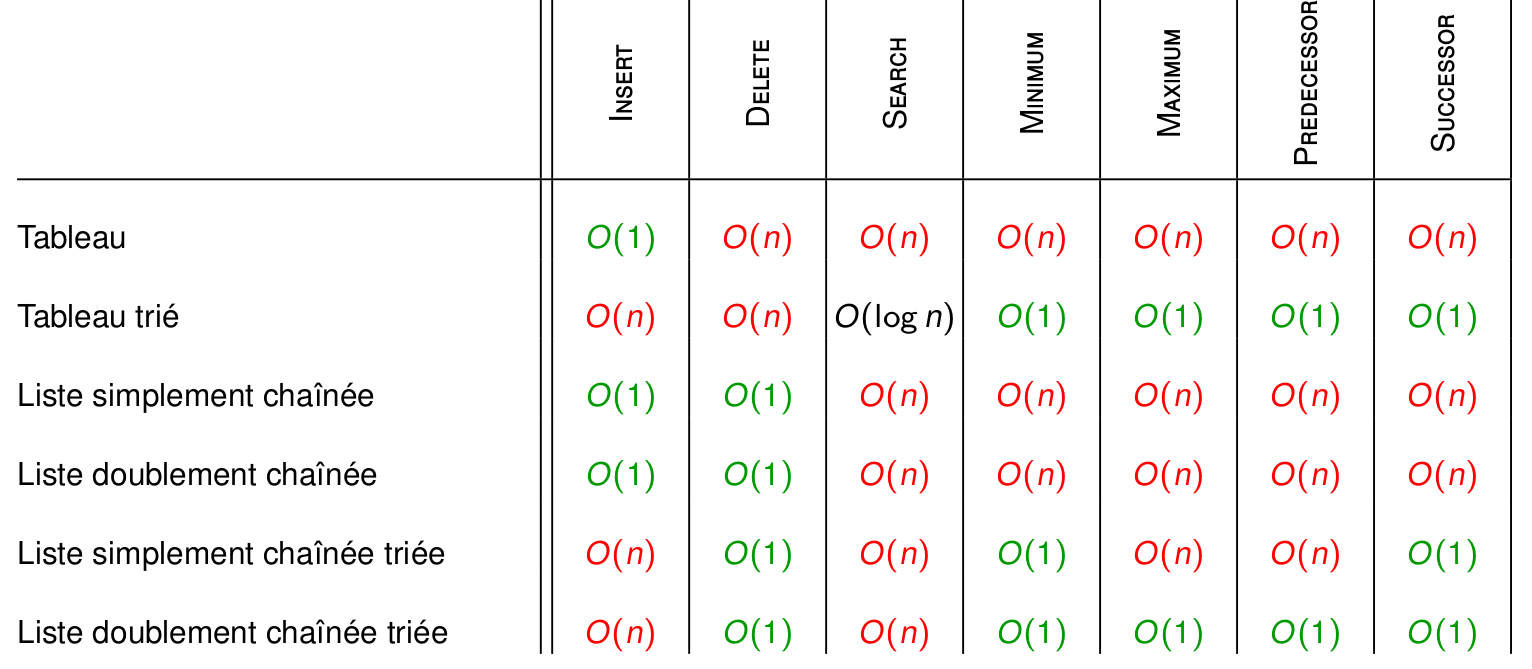
\includegraphics[width=0.9\linewidth]{comparaison_structures.png}
\caption{Comparaison des coûts des opérations classiques entre les structures de données connues.}
\label{fig:comparaison_structures}
\end{figure}
Nous allons dans ce cours voir trois nouvelles structures de données : les \textbf{tas-max}, les \textbf{arbres binaires de recherche}, et les \textbf{tables de hachage}.
\section{Tas-max et queue de priorité}
\bg{Disclaimer}{Quand on dit "max" et "maximum", tout le raisonnement se fait également en disant "min" et "minimum".}
\subsection{Queue de priorité max}
Une queue de priorité \textbf{max} est un type de données abstrait dont les opérations à faire supporter sont les suivantes :
\begin{center}
\begin{tabular}{r|p{10cm}}
     \code{Insert(S,x)} & Insérer l'élément \code{x} dans la queue \code{S}. \\\rule{0pt}{20pt}
     \code{Maximum(S)} & Renvoie l'élément de \code{S} avec la plus grande clé.\\\rule{0pt}{20pt}
     \code{Extract-Max(S)} & Renvoie  et supprime l'élément de \code{S} avec la plus grande clé. \\\rule{0pt}{20pt}
     \code{Increase-Key(S,x,k)} & Augmente la valeur de la clé de l'élément \code{x} jusqu'à la nouvelle valeur \code{k} (devant être supérieure à l'ancienne valeur).      
\end{tabular}
\end{center}
Aucune structure de données déjà vue (présente sur la structure \ref{fig:comparaison_structures}) permet d'effectuer ces opérations en un temps acceptable (constant ou $\Theta(\log(n))$). Il nous faut une nouvelle structure de données, et il est temps d'introduire notre première structure de donnée inédite : les \textbf{tas-max}.
\subsection{Tas}
Un tas est une structure de données implémentée par un tableau et qui peut être visualisé sous la forme d'un arbre binaire (presque complet). Pour le parcourir, la notice est présentée à la figure \ref{fig:tas_parcours}. Cette structure de donnée permettra, une fois complétée de certaines propriétés, d'effectuer \textbf{toutes les opérations de la queue de priorité en un temps $O(\log(n))$}.

\begin{figure}[h]
\centering
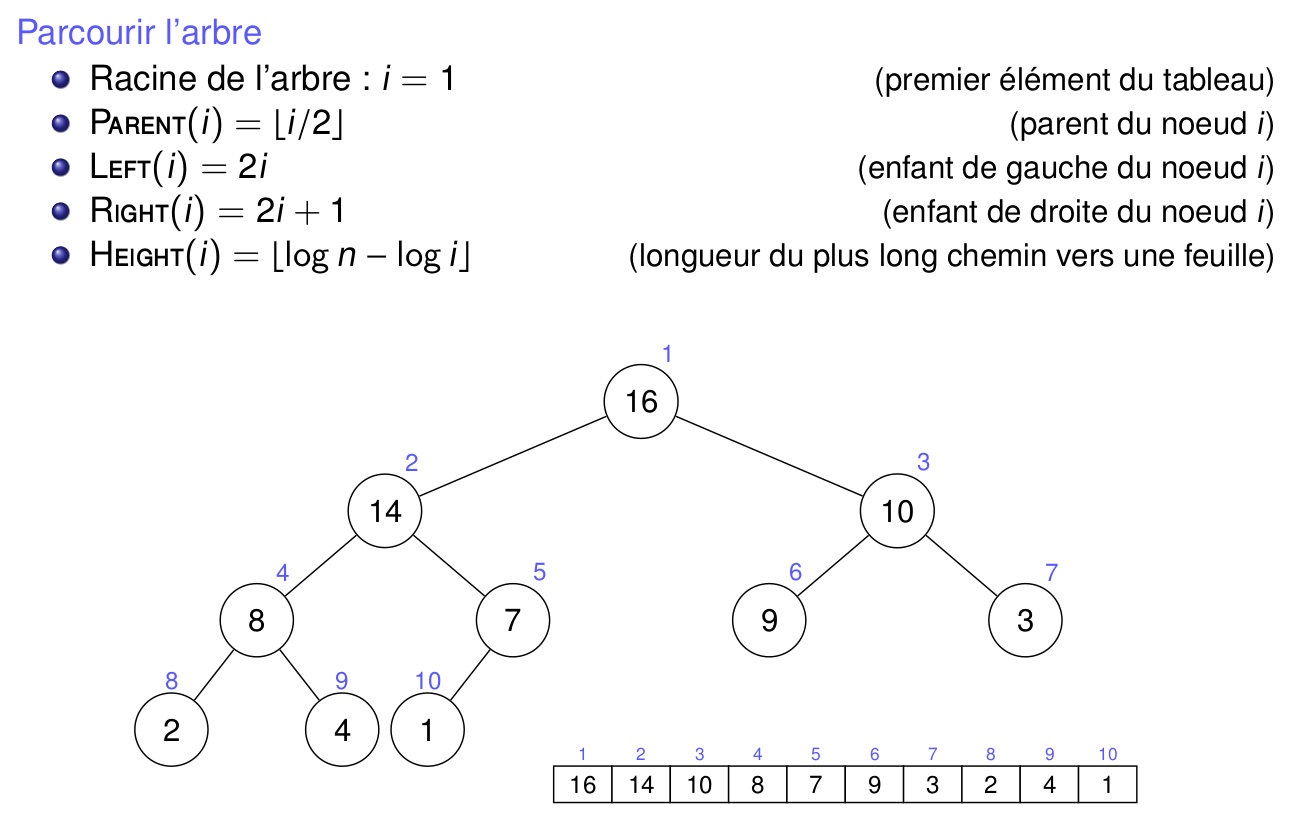
\includegraphics[width=0.8\linewidth]{tas_parcours}
\caption{Parcours d'un tax}
\label{fig:tas_parcours}
\end{figure}
\subsection{Tas-max}
Un tax-max est un tas tel que $$A\left[\text{\textsc{Parent}}(i)\right] \geq A[i] \quad \forall i \neq \text{\textsc{Root}}$$

\subsubsection{Opérations à implémenter}
\begin{center}
\begin{tabular}{|l|}

\hline
Construction et maintien d'un tas-max \\
\hline \\
\begin{tabular}{p{5cm}|p{10cm}} 
     \rouge{\textsc{Build-Max-Heap}} & construit un tas-max à partir d'un tableau désordonné. \\\rule{0pt}{20pt}
     \rouge{\textsc{Max-Heapify}} & corrige une violation unique de la prorpriété de tas 
\end{tabular} \\ \rule{0pt}{20pt} \\
\hline
\hline
Opérations de queue de priorité \\
\hline \\
\begin{tabular}{p{5cm}|p{10cm}}\rule{0pt}{20pt} 
     \rouge{\textsc{Heap-Maximum}} & renvoie l'élément avec la plus grande clé. \\\rule{0pt}{20pt}
     \rouge{\textsc{Heap-Extract-Max}} & renvoie et supprimer l'élément avec la plus grande clé 
\end{tabular} \\ \rule{0pt}{20pt} \\
\hline 
\hline
Opérations de tri \\
\hline \\
\begin{tabular}{p{5cm}|p{10cm}}
     \rouge{\textsc{Heapsort}} & trier un tableau en place. 
\end{tabular} \rule{0pt}{20pt}\\ \hline
\end{tabular}
\end{center}
\subsubsection{\pseudo{Max-Heapify}}
Cette méthode consiste à corriger une violation \textbf{unique} de la propriété de tas. Un noeud peut vérifier la propriété de tas sans pour autant que ses enfants la vérifient ! \\

Si un noeud $i$ viole la propriété de tas-max, c'est qu'un de ses enfants est plus grand que lui. L'idée sera alors d'échanger l'élément au noeud $i$ par son plus grand enfant, et vérifier qu'on n'a pas ce faisant généré une violation au noeud échangé. 
\begin{figure}[h]
\centering
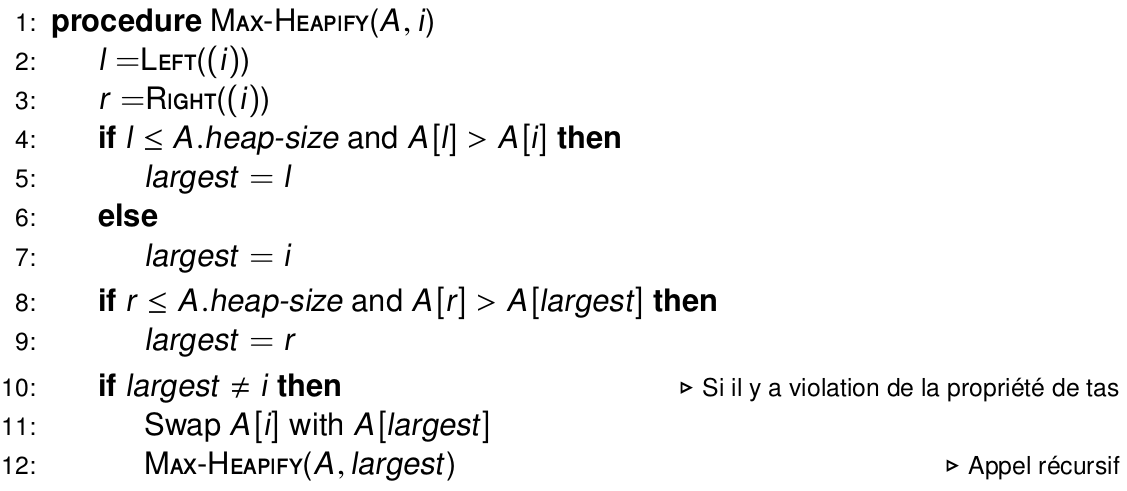
\includegraphics[width = 0.7\linewidth]{max-heapify_pseudoc}
\caption{Pseudo-code de l'opération de correction d'une violation unique de la propriété de tas-max, \rouge{\textsc{Max-Heapify}}}
\label{fig:max-heapify_pseudoc}
\end{figure}
La complexité de cette méthode s'évalue facilement : on a une récurrence 
$$\begin{array}{rl}
\text{Cas de base :} \quad T(0) &= c \\
T(h) &= c + T(h-1) \\
\Rightarrow T(h) &= c + h\cdot c
\end{array}$$
où $h$ est la hauteur du noeud $i$. Celle-ci est toujours inférieure à $\log(n)$, il est donc correct de conclure en disant que \rouge{\textsc{Max-Heapify}} a une complexité en $O(\log n)$, car
$$\text{\pseudo{Height}}(i) = \lfloor \log(n) - \log(i) \rfloor \leq \log(n)$$
\subsubsection{\pseudo{Build-Max-Heap}}
Le but est ici de corriger dans un tas \textbf{toutes les violations} de la propriété de tas, pas juste celle à un noeud. On va alors parcourir toutes les feuilles et appliquer la méthode \pseudo{Max-Heapify} sur chacun des noeuds parents pour vérifier que la propriété est respectée et de la faire respecter si non. On va donc commencer depuis le \textbf{parent du dernier élément}, à savoir 
$$\pseudo{Parent}(n) = \lfloor n/2 \rfloor$$
\begin{figure}[h]
\centering
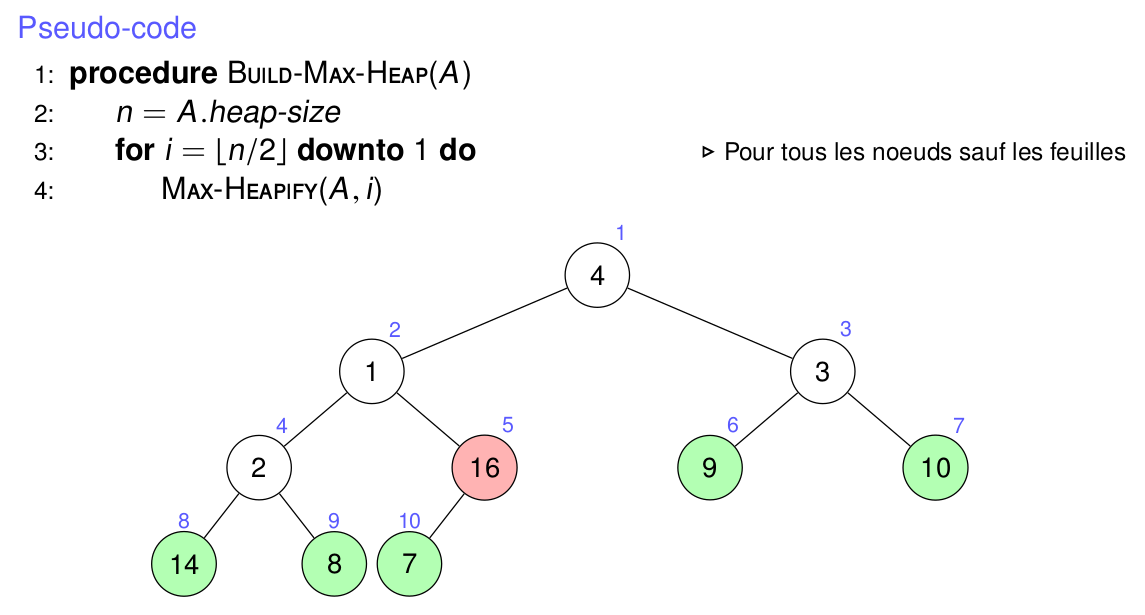
\includegraphics[width=0.8\linewidth]{build-max-heap_pseudoc}
\caption{Pseudo-code de l'opération \pseudo{Build-Max-Heap} qui consiste à construire un tas-max à partir de n'importe quel tas désordonné.}
\label{fig:build-max-heap_pseudoc}
\end{figure}
On va donc appliquer \pseudo{Max-Heapify} sur chacun des noeuds de l'arbre, soit $\lfloor n/2 \rfloor$ noeuds. Le coût de \pseudo{Max-Heapify} vaut dans le pire des cas $\Theta(h)$ pour un noeud à la hauteur $h$, donc $O(\log(n))$. La complexité de \pseudo{Build-Max-Heap} est donc en $O(n\cdot \log(n))$. \\

Une analyse plus fine est obtenue, comme avant, en sommant ce qu'il y a à sommer. À chaque étage de hauteur $h$, il y a environ $\frac{n}{2^{h+1}}$ noeuds. Et pour chaque noeud à la hauteur $h$, le traitement de ce noeud prend un temps linéaire selon $h$ : $T_h = c\cdot h$. Le coût total est alors obtenu en sommant sur chaque hauteur, de $h=1$ à $h=\log(n)-1$.

$$\begin{array}{ll}
T(n) &= \sum_{h=1} ^{\log(n)-1} \dfrac{n}{2^{h+1}} \cdot c \cdot h \\
&= \dfrac{c\cdot n}{2}\sum_{h=1} ^{\log(n)-1} \dfrac{h}{2^h} \\
&= \Theta(n)
\end{array}$$
Et c'est ainsi qu'on démontre non seulement que la vraie complexité de la construction d'un tas-max est $\Theta(n)$ et non $O(n\cdot \log(n))$ et que la création d'un tas-max prend exactement le même temps que créer un tableau désordonné de $n$ éléments.
%Sauf que cette analyse est \textbf{pessimiste} parce qu'elle considère le pire cas pour chaque noeud. Or il se peut qu'on soit à une feuille à la hauteur $h$, ce qui est tout de suite moins coûteux !

\subsubsection{\pseudo{Extract-Max}}
Le maximum se trouve à la racine. On pourrait le supprimer directement en créant un trou dans l'arbre, mais ce n'est pas trop ce qu'on a envie de faire. Pour ne pas créer de trou, on préfère remplacer la racine par le dernier élément, puis d'appliquer \pseudo{Max-Heapify} sur la racine.
\begin{figure}[h]
\centering
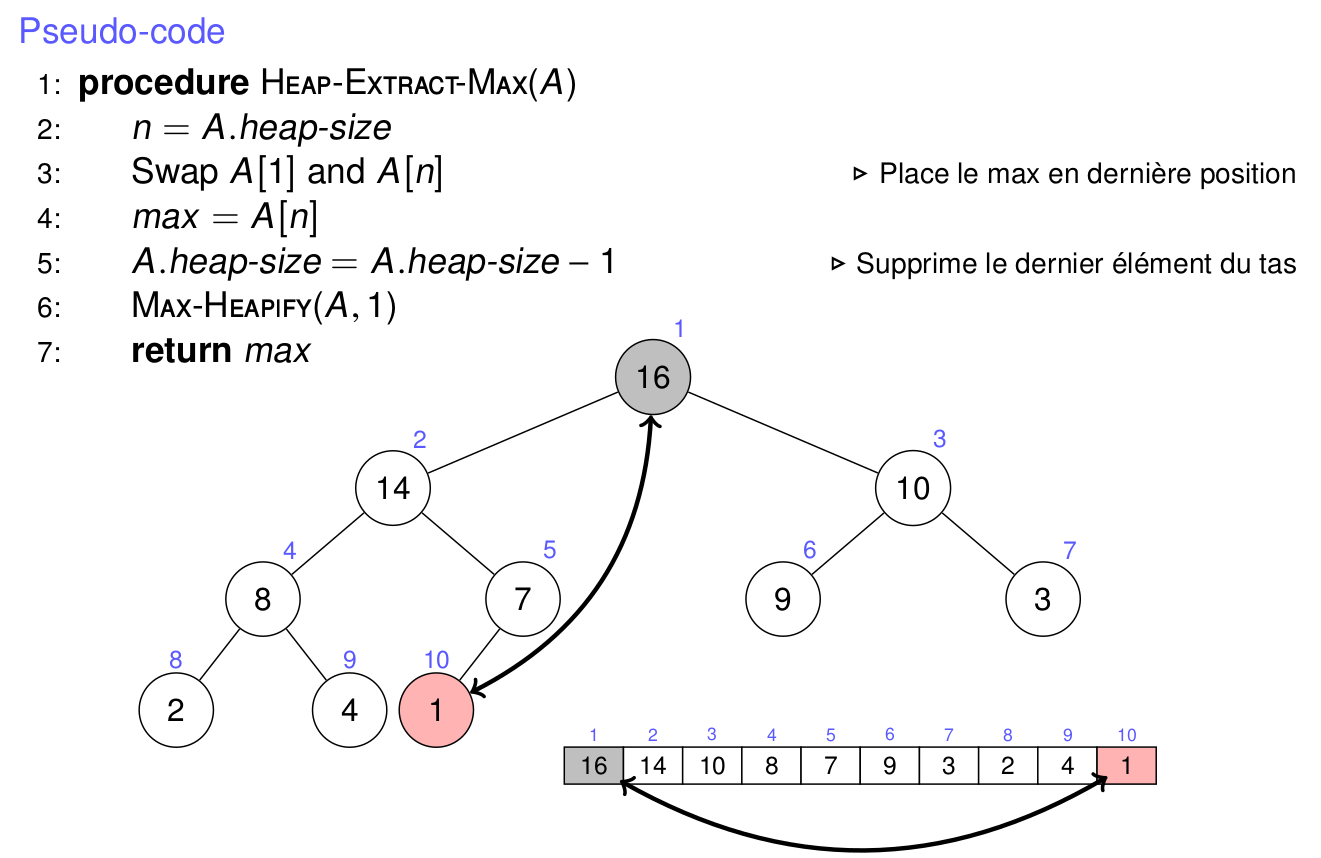
\includegraphics[width=0.8\linewidth]{extract-max.png}
\caption{Pseudo-code de la méthode \pseudo{Extract-Max}}
\label{fig:extract-max}
\end{figure}
La complexité de cette méthode s'évalue simplement : une permutation de deux éléments $\Theta(1)$ et appeler \pseudo{Max-Heapify} sur la racine de hauteur $\log(n)$ d'où un coût en $\Theta(\log(n))$.
\subsection{Tri par tas (heapsort)}
Le tri par tas consiste à profiter de la structure d'un tas-max pour trier un tableau désordonné. Comme on l'a déjà vu, pour le transformer en tas, il faut appliquer \pseudo{Build-Max-Heap} ce qui prend un temps $\Theta(n)$. Ensuite, pour trier ce tas, on a vu qu'on pouvait extraire le maximum avec \pseudo{Extract-Max} en un temps $\Theta(\log(n))$ en l'échangeant avec le dernier élément du tableau (dernier en termes d'indices). En appliquant \pseudo{Extract-Max} $n$ fois, on aura trié le tableau. \\

La complexité d'un tri par tas est donc en $\Theta(n\cdot \log(n))$ soit la même que le tri par fusion. L'avantage ici est que le tri est 100\% en place.

\bb{Tri par tas : $T(n) = \Theta(n\cdot \log(n))$ et en place}


\section{Choix et conception d'une structure de données}
À chaque application sa structure de données propre. Afin de la choisir, il faut, dans l'ordre :
\begin{enumerate}
\item Déterminer les opérations nécessaires (spécification du type de données abstrait)
\item Choisir une structure de données appropriée (qui limite le coût des opérations nécessaires)
\item Implémenter la structure de données
\item Débuguer
\end{enumerate}
Pour débuguer, il faut faire appel à la notion d'\textbf{invariant de représentation}.
\subsection*{Invariant de représentation}
Un invariant de représentation est une propriété d'une structure de données qui reste vérifiée à tout moment de l'exécution. Ca peut être l'ordre pour un tableau trié, la propriété de tas pour un tas-max, ... \\

Une erreur lors de l'implantation d'une opération peut violer cet invariant et provoquer d'autres bugs par la suite. Une bonne stratégie de débugage serait alors d'implémenter une méthode qui vérifie si l'invariant est toujours respecté, et de l'appliquer avant et après certaines opérations pour localiser où surviendrait la potentielle couille qui rend le potage légèrement aigre.
\section{Taille de tableau}
Généralement, on crée un tableau (sur base d'une certaine structure) et puis on le complète. On lui fixe une taille dans la mémoire à sa création, mais il se peut qu'on soit un peu trop prévoyant et qu'on prévoie $m$ places pour au final remplir $n\ll m$ éléments. En outre, si nous voulons ajouter un élément et qu'on se rend compte qu'on dépasse la taille prévue, il faut créer un autre tableau plus grand en mémoire et copier l'ancien tableau dans le nouveau, ce qui prend un temps $\Theta(n)$. De même si l'on supprime beaucoup d'éléments : on aura peut-être pour finir un gros emplacement non utilisé en mémoire, ce dont il faut s'occuper en créant un tableau plus petit. On se retrouve encore avec du $\Theta(n)$.\\

Dans cette section, on cherche à optimiser à la fois la place occupée en mémoire et le temps passé à faire ces opérations de création de nouveaux tableaux.

\subsection{Stratégie lors de l'insertion -- doublement de tableau}
Il faut déterminer une règle pour redimensionner le tableau.
\subsubsection{Approche naïve}
 L'approche naïve consiste à dire qu'à chaque insertion on crée un tableau de taille $m'$ tel que 
$$m' = m+1$$
Cela veut dire qu'à chaque insertion, on doit effectuer un redimensionnement et donc une copie du tableau vers un nouveau en mémoire. En commançant avec un tableau de taille $1$, puis $2$, puis $2 + \cdots + n$ pour ajouter $n$ éléments. On calcule le temps pris pour l'insertion de $n$ éléments :
$$\Theta(1+2+\cdots+n) = \Theta\left(\dfrac{n(n+1)}{2}\right) = \Theta(n^2)$$
Cela donne donc en moyenne $\Theta(n)$ par insertion. 

\subsubsection{Doublement de tableau}
Le doublement de tableau consiste à \textbf{redimensionner le tableau à chaque fois que $n$ est multiplié par 2}. À chaque fois :
$$m' = 2 \cdot m \; .$$
Ainsi, le surcoût dû aux redimensionnements est calculé selon :
$$\Theta(1 + 2 + 4 + \cdots + n) = \Theta\left( \sum_{i=0} ^{\log(n)} 2^i \right) = \Theta(n)$$
Donc un coût "moyen" par insertion de $\Theta(1)$. On dit que la méthode \pseudo{Insert} a un coût \textbf{amorti} de $\Theta(1)$. Le redimensionnement n'implique pas de surcoût en moyenne.

\subsection{Stratégie à la suppression}
Il faut également redimensionner le tableau lors de la suppression d'un grand nombre d'éléments. Typiquement, on aimerait, pour un tableau de taille $m$ rempli de $n$ éléments, maintenir la propriété suivante :
$$C \cdot m \leq n \leq m \quad , \; C < 1  \; ,$$
et il faut choisir cette constante. \\
Si nous choisissons $C = 1/2$, alors la taille du tableau diminue de moitié lorsque la moitié manquera. Cependant, si nous voulons ajouter un élément juste après, alors il faudra réagrandir le tableau si on suit le critère précédent. $n$ suppresions/insertions provoquera donc $n$ redimensionnements, soit un coût total en $\Theta(n^2)$ ou un coût amorti en $\Theta(n)$. \\

Si nous choisissons $C = 1/4$, alors on a quelque chose de bien plus beau, car il faudra réinsérer $m'/2$ éléments avant de devoir redimensionner. Le coût amorti restera donc en $\Theta(1)$.

\section{Arbres de recherche}
\section{Tables de hachage}

\part{Techniques de programmation}
\chapter{Backtracking}
Nous revenons au but de la vie de l'ingénieur : résoudre des problèmes. Quand on accepte que les ordinateurs fassent partie de notre formidable vie, on fait aussi le choix de les laisser gérer nos problèmes du quotidien pour nous (sauf ceux avec les femmes, malheureusement aucun algorithme assez puissant peut nous sortir de la merde avec elles). Si il existe plusieurs solutions pour répondre à un problème, l'algorithme va \textbf{toutes les trouver}. Mais s'il y a plusieurs possibilités sans pour autant qu'elles soient toutes possibles, l'algorithme va quand même devoir toutes les essayer, ce qui prendrait un temps fou ! À moins qu'interviennent les humains intelligents qui mettent en place des techniques splendides pour optimiser le calcul. Parmi elles, \textbf{le backtracking}. \\

Très brièvement, le backtracking consiste à rechercher une solution en essayant plusieurs voies, et revenir en arrière lorsqu'une de ces voies s'avère incorrecte, et alors choisir une autre.
\section{Génération exhaustive}
Ce concept est le plus idiot et chronophage possible, et on se demande à quoi elle sert parce qu'il ne s'agit pas de résoudre un problème, il s'agit de lister tous les candidats possibles et imaginables. Le pseudo-code de la génération exhaustive est présent sur la figure \ref{fig:generation-exhaustive_pseudoc}.
\begin{figure}[h]
\centering
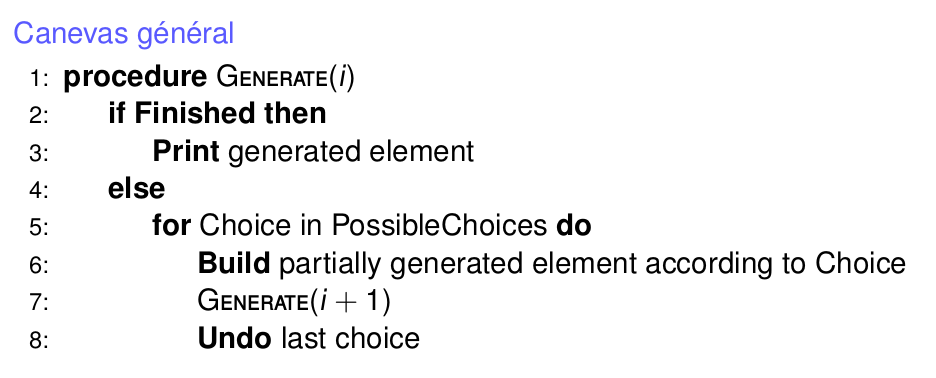
\includegraphics[width=0.8\textwidth]{generation-exhaustive_pseudoc}
\caption{Pseudo-code de la génération exhaustive, en ayant en tête une chaîne que l'on remplit progressivement jusqu'à une taille $n$. Lorsque $i=n$ on est dans la situation \pseudo{Finished}}
\label{fig:generation-exhaustive_pseudoc}
\end{figure}
On utilise déjà là en réalité le backtracking puisqu'à chaque position on entame une nouvelle version de la chaîne à partir de l'élément d'après (\pseudo{Generate}(i+1)) mais on fait un \pseudo{Undo} pour revenir en arrière et prendre un nouveau choix qui va mener à une différente situation d'arrivée.
\section{Recherche exhaustive}
La \textbf{recherche exhaustive} est premièrement un poil plus exigeante que la génération exhaustive car elle ne demande d'imprimer que les candidats qui sont solutions. Ensuite, il advient en toute logique que nous n'aimerions pas explorer des pistes qui ne mènent de toute façon pas à de bons résultats. Sur base de notre situation, nous seront amenés à définir des critères qui consisteront à dire si un choix est admissible ou non. Un canevas de recherche exhaustive optimisée est représenté sur la figure \ref{fig:recherche-exhaustive_pseudoc}.
\begin{figure}[h]
\centering
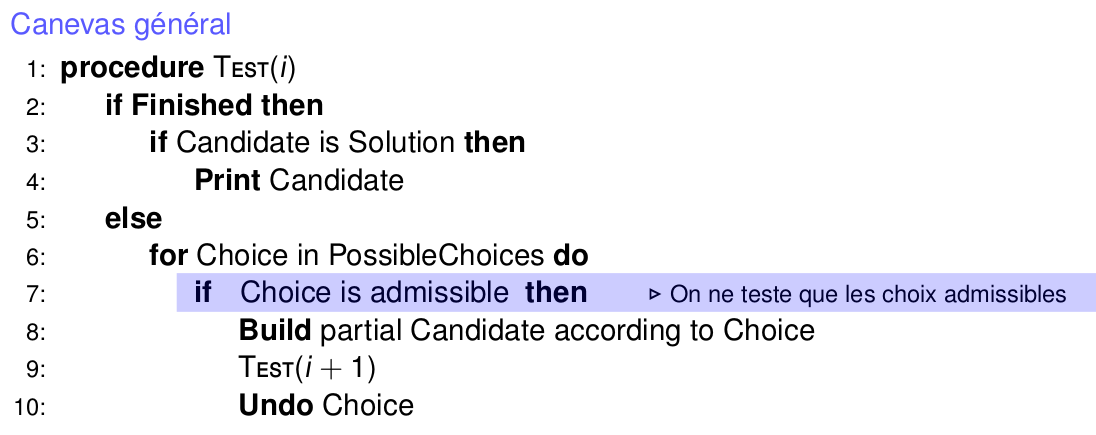
\includegraphics[width=0.8\textwidth]{recherche-exhaustive_pseudoc}
\caption{Pseudo-code de la recherche exhaustive, où la notion de \textbf{choix admissible} apparaît, contrairement à la génération exhaustive où la seule notion intéressante était la notion de \textbf{choix possible}.}
\label{fig:recherche-exhaustive_pseudoc}
\end{figure}


\section{Recherche d'une seule solution}
On commence ici à modifier les pseudo-codes précédents en y incluant la possibilité qu'une solution soit trouvée. Pour rappel, jusque là, on appliquait la méthode \pseudo{Test} récursivement sur la position $i$ de la chaîne en augmentant $i+1$ à chaque appel, jusqu'à arriver à $i=n$ où la chaine est terminée et on vérifie si la proposition candidate est solution ou non. \\

Maintenant, on ajoute les \textbf{retours} de la fonction : à chaque fois qu'on arrive à $i=n$, si on a une solution on renvoie \code{true}, sinon on renvoit \code{false}. Ensuite, pour chaque appel récursif \pseudo{Test}$(i+1)$, on retourne \code{true} si le choix qu'on a effectué mène à un chemin qui mène à une solution, false sinon. Le canevas général de la recherche d'une solution est affiché sur la figure  \ref{fig:recherche-exhaustive_pseudoc}

\begin{figure}[h]
\centering
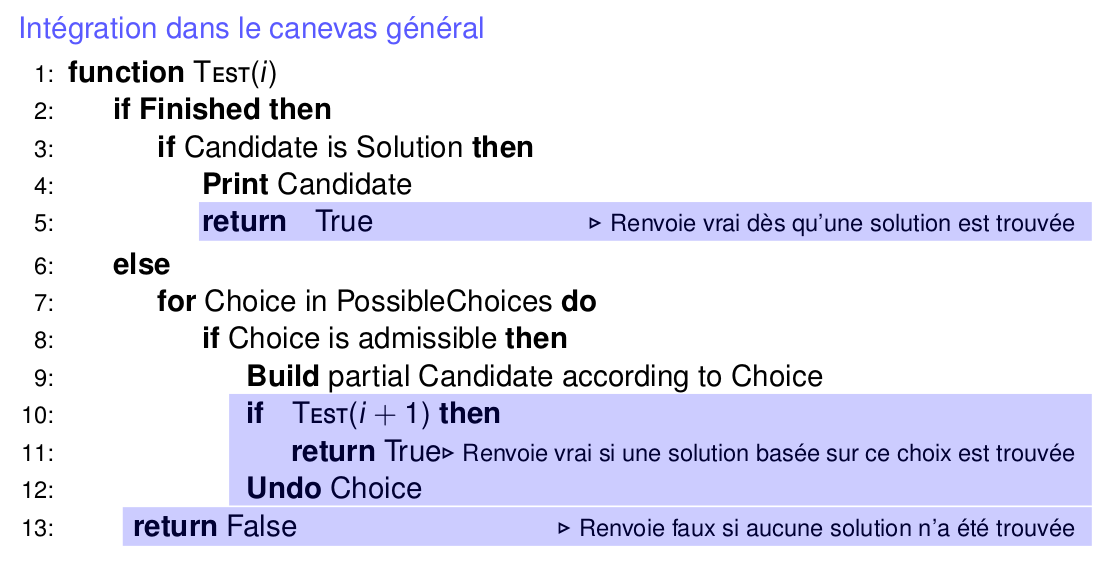
\includegraphics[width=0.8\linewidth]{recherche-solution_pseudoc}
\caption{Pseudo-code de la recherche exhaustive d'une solution en général.}
\label{fig:recherche-solution_pseudoc}
\end{figure}
\bg{Exemple}{
Pour le problème de remplissage d'un sac, la figure ci-dessous reprend le pseudo-code de la recherche d'une solution. On remarque par exemple que le critère d'admission d'un choix se base sur le débordement ou non du sac lors de l'ajout de l'objet en question. S'il peut être ajouté, alors on l'ajoute et on vérifie que ça mène peut-être à une solution. Si ça mène en effet à une solution (\pseudo{Test}$(i+1)$ renvoie \code{true}), la fonction s'arrête en renvoyant \code{true}. Si non, on fait une \textbf{marche arrière} (lignes 12 et 13) et on enlève l'objet du sac. On vérifie que ne pas mettre l'objet dans le sac permet en effet de résoudre le problème et si c'est le cas la fonction renvoie \code{true}, sinon elle renvoie \code{false}.
\begin{center}
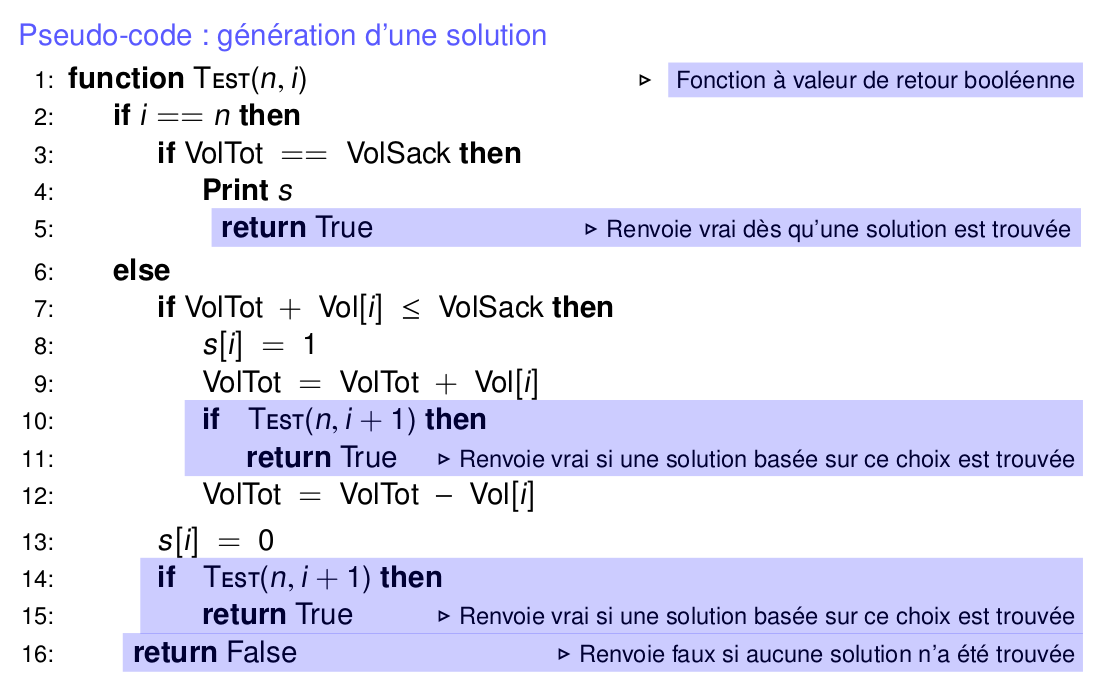
\includegraphics[width=0.8\linewidth]{recherche-exhaustive_exemple}
\end{center}
}
\section{Recherche de la meilleure solution}
Si on désire rechercher la meilleure solution, il suffira de sauvegarder chaque solution trouvée dans une variable temporaire et de l'écraser par une nouvelle solution arrivante si cette-dernière est meilleure. Le pseudo-code serait alors celui de la figure \ref{fig:recherche-meilleure-solution_pseudoc}
\begin{figure}[h]
\centering
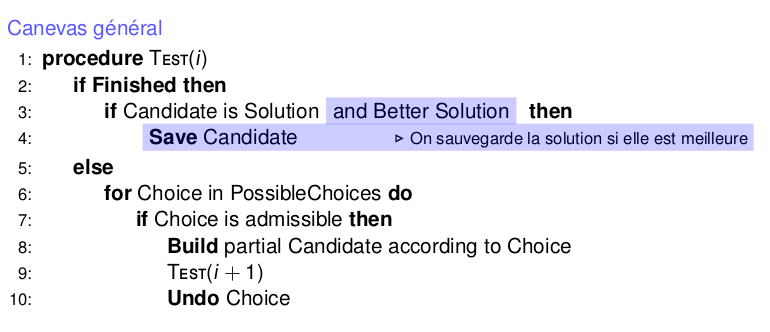
\includegraphics[width=0.8\linewidth]{recherche-meilleure-solution_pseudoc}
\caption{Pseudo-code de la recherche de la meilleure solution d'un problème.}
\label{fig:recherche-meilleure-solution_pseudoc}
\end{figure}

\section{Branch-and-bound}
La recherche d'une meilleure solution par recherche exhaustive passe tout de même par un semblant de génération exhaustive d'un nombre potentiellement exponentiel de candidats. Le coût est donc \textbf{typiquement exponentiel}. Comme on est jamais content, on est pas content là non plus. Il faut venir avec une nouvelle technique. \\

Le \textbf{branch-and-bound} est une technique qui consiste à réduire le coût en évitant de générer certains candidats, typiquement ceux qui ne mèneraient pas à une meilleure solution. On ne vérifie donc pas seulement que le choix est admissible, mais qu'il ne puisse pas donner un résultat moins bon que la meilleure solution initialement trouvée. Si il peut mener à une meilleure solution, alors on applique \pseudo{Test} à $i+1$.
\begin{figure}[h]
\centering
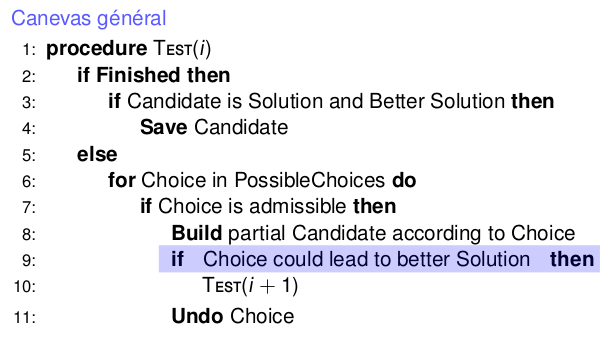
\includegraphics[width=0.8\textwidth]{branch-and-bound}
\caption{Pseudo-code de la méthode de branch-and-bound}
\label{fig:branch-and-bound}
\end{figure}

\chapter{Programmation dynamique}
\section{Bilan de mi-parcours}
Nous avons vu les 5 étapes de conception d'un algorithme en programmation dynamique :
\bo{\textsc{Etapes de conception -- Programmation dynamique}
\begin{enumerate}
\item Déterminer les "choix" pour construire une solution partielle
\item Définir les sous-problèmes
\item Relier les solutions des sous-problèmes entre elles (relation de récurrence)
\item Concevoir l'algorithme proprement dit : soit à partir de la formule de récurrence (algorithme récursif avec mémoïsation), soit en établissant le graphe de dépendance (algorithme de bas en haut)
\item Résoudre le problème initial (fonction principale)
\end{enumerate}}
\subsection{Types de sous-problèmes}
Nous allons voir qu'on a des types de sous-problèmes qui reviennent souvent et qu'on peut classifier. Remarquons déjà qu'en général, un problème traité en programmation dynamique peut se modéliser via un tableau comme ça l'a toujours été jusqu'à présent. Considérons un tableau $T[0:n-1]$. Il y aura comme possibilité de sous-problèmes :
\begin{table}[h]
\centering
\begin{tabular}{c|c|c}
Type & Description & \# sous-problèmes \\ 
\hline \rule{0pt}{20pt}
\bleu{Suffixes} &  $T[i:n-1]$ pour tout $i$ & $n$ \\\rule{0pt}{20pt}
\bleu{Préfixes} & $T[0:i]$ pour tout $i$ & $n$ \\\rule{0pt}{20pt}
\bleu{Sous-tableaux} & $T[i:j]$ pour tous $i\leq j$ & $\sim n(n+1) = \Theta(n^2)$
\end{tabular}
\caption{Types de sous-problèmes à traiter les de la résolution d'un problème par une technique de programmation dynamique.}
\label{tab:progDyn_soustableaux}
\end{table}

\section{Exemples avancés}
\subsection{Parenthésage}
Le problème de parenthésage concerne la multiplication matricielle, et plus précisément lorsque nous sommes amenés à évaluer une multiplication d'une chaîne de matrices, soit 
$$M = A_1 \cdot A_2 \cdot ... \cdot A_{n-1} \cdot A_n$$
et que nous cherchons à \textbf{établir le parenthésage} qui rende la multiplication plus rapide. Il s'agit en gros de l'endroit où séparer deux termes d'une paire de parenthèses dans le calcul de $M$ (et de même pour la séparation en deux termes de chaque terme). On peut en effet montrer en prenant l'exemple $$M = A_1 \cdot A_2 \cdot A_3$$ où
\begin{itemize}
\item $A_1$ est de taille $\bleu{n}\times \rouge{1}$ (matrice colonne)
\item $A_2$ est de taille $\rouge{1}\times \green{n}$ (matrice ligne)
\item $A_3$ est de taille $n\times 1$ (matrice colonne)
\end{itemize}
qu'il existe un parenthésage optimal. En effet, si nous considérons le parenthésage $(A_1 \cdot A_2) \cdot A_3$, le coût du calcul de $M_1 = A_1\cdot A_2$ vaut $\bleu{n} \cdot \rouge{1} \cdot \green{n} = n^2$ et celui de $M = M_1 \cdot A_3$ vaudra $n^2 n \cdot n \cdot 1 = n^2$. Le coût de la multiplication en chaîne de ces 3 matrices sera en $\Theta(n^2)$. \\

Si nous choisissons en revanche l'option qui consiste à calculer d'abord $A_2\cdot A_3$, alors nous arriverons à diminuer le coût total. En effet : le coût pour $M_2 = A_2\cdot A_3$ (scalaire de taille $\rouge{1}\times \underline{1}$) est de $1\cdot n \cdot 1$ et celui de $A_1 \cdot M_2$ sera de $\bleu{n} \cdot \rouge{1} \cdot \underline{1} = \Theta(n)$ ce qui est meilleur que $\Theta(n^2)$ !

\subsubsection{Les 5 étapes}
Nous allons maintenant décrire le problème de parenthésage général et l'explorer par la méthode de programmation dynamique, en commençant d'abord par l'analyser selon les 5 étapes. \\
\begin{enumerate}
\item \textbf{Choix.} \\
Par "choix", nous entendons la chose suivante. Nous voyons le problème global :
\leftbar[0.9\textwidth]
\begin{center}
$M = A_1 \cdot A_2 \cdot ... \cdot A_{n-1} \cdot A_n$ dont le coût est à optimiser en calculant au préalable deux termes : c'est-à-dire effectuer le produit 
$$M = (A_1 \cdot A_2 \cdot ... \cdot A_j)\cdot (A_{j+1} \cdot A_{j+2} \cdot ...  \cdot A_n)$$
\end{center}
\endleftbar
Le choix suivant consiste à optimiser le calcul des deux termes par la même méthode :
$$((A_1 \cdot ... \cdot A_{i-1}) \cdot (A_i \cdot ... \cdot A_j))\quad \cdot \quad ((A_{j+1} \cdot ... \cdot A_{k}) \cdot (A_{k+1} \cdot ... \cdot A_{n}))$$

\item \textbf{Sous-problèmes.} \\
Les sous-problèmes du premier choix sont consistués de suffixes et de préfixes. A partir du deuxième choix, on se retrouve avec \textbf{tous les sous-tableaux} $$A_i \cdot ... \cdot A_j \qquad \forall 1 \leq i \leq j \leq n \; .$$
On a donc $\Theta(n^2)$ sous-problèmes (cf. table \ref{tab:progDyn_soustableaux}). Et pour chacun de ces problèmes, on a $j-i \leq n$ choix possibles. \\

\item \textbf{Récurrence.} \\
Si nous notons $P_{i:j}$ le coût du \textbf{parenthésage optimal} (et non du produit matriciel!) pour le problème 
$$A_i \cdot ... \cdot A_j = (A_i \cdot ... \cdot A_k) \cdot (A_{k+1} \cdot ... \cdot A_j)$$
On obtient aisément la récurrence suivante :
$$P_{i:j} = \min_{i\leq k \leq j} \left\{ \text{Cost}(i,j,k) + P_{i:k} + P_{k+1:j} \right\} \qquad \forall 1 \leq i \leq j \leq n $$
où cette fois $\text{Cost}(i,j,k)$ est le coût du produit matriciel, qui dépend des dimensions de $A_i,A_k, A_j$. \\

Le cas de base correspond à un produit avec une seule matrice, ce qui prend un temps constant, d'où $$P_{i:i} = 0 \qquad \forall i \; .$$
Par sous-problème, on a toujours $j-i$ choix possibles, d'où

$$\boxed{\text{Coût/sous-pb.} \quad O(j-i) = O(n)} \; .$$

\item \textbf{Graphe de dépendance.} \\
Enfin, si l'on trace le graphe de dépendance pour dérécursifier l'algorithme, on voit les dépendances suivantes, en simplifiant le graphe sur la figure \ref{fig:progDyn_parenth_graphe_dependance}. \\
\begin{figure}[h]

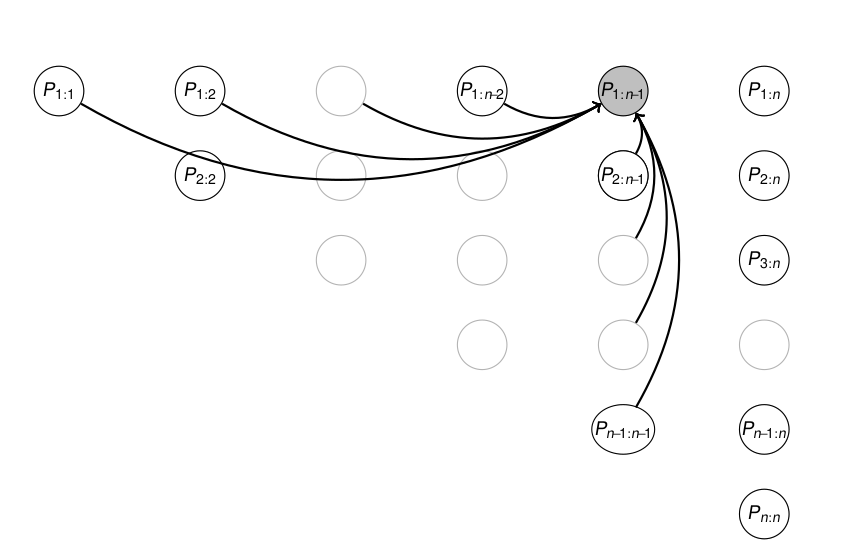
\includegraphics[width=0.5\textwidth]{progDyn_parenth_graphe_dependance} \hspace{1cm} 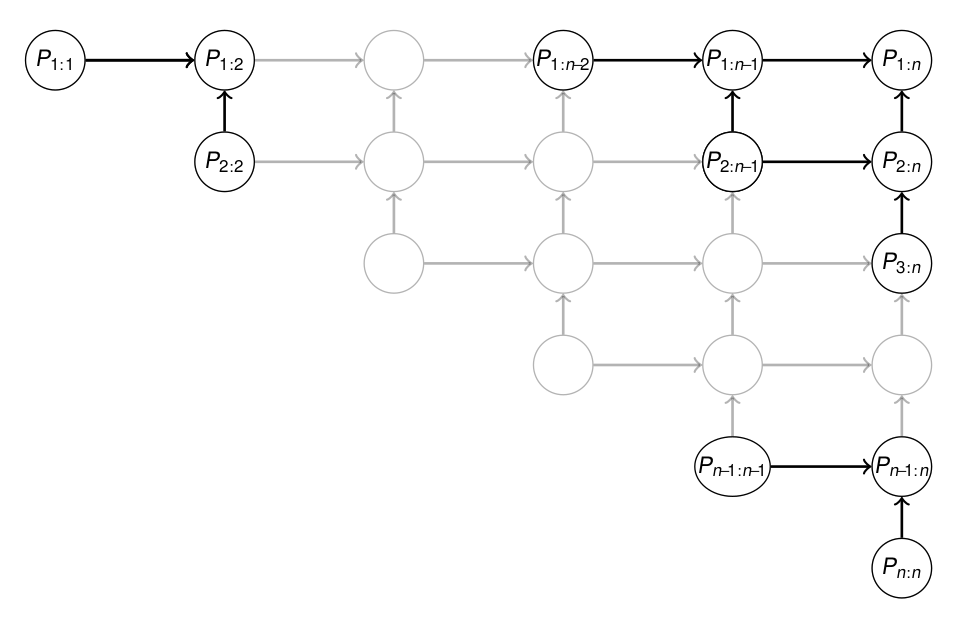
\includegraphics[width=0.5\textwidth]{progDyn_parenth_graphe_dependance2}
\caption{Graphe de dépendance avec une version simplifiée.}
\label{fig:progDyn_parenth_graphe_dependance}
\end{figure}

\item \textbf{Problème initial.} \\
Pour retourner au problème initial, qui est $P_{1:n}$, on a $\Theta(n^2)$ sous-problèmes, $O(n)$ pour le coût d'un sous-problème et un coût constant pour le problème initial, ce qui revient à un coût de $O(n^3)$ pour le coût total de la solution du problème de parenthésage optimal.
\end{enumerate}
\subsection{Plus longue sous-séquence commune}
Par sous-séquence, nous entendons "partie d'un mot dont tous les caractères se trouvent dans le même ordre dans le mot". Le problème de la plus longue sous-séquence commune est le suivant. \\

On se donne deux chaînes de caractères et on cherche une chaîne de caractère qui soit à la fois une sous-séquence du premier et du deuxième. On recherche plus précisément la \textbf{plus longue}. La solution n'est pas forcément unique ! Le problème a l'air abstrait mais a une application typique, par exemple la comparaison de chaînes ADN.

\subsubsection{Résolution en programmation dynamique -- les 5 étapes}
Si on commence à l'étape 2, on identifie les sous-problèmes : des suffixes, préfixes, ou des sous-tableaux. La différence ici est qu'on a deux tableaux, $s$ et $t$. Pour deux chaînes, on va \textbf{supposer dans un premier temps que les sous-problèmes sont représentés par des suffixes} (on va le montrer). Alors on a les suffixes suivants pour les premiers sous-problèmes :
$$s[i:n-1] \qquad t[j:n-1]$$
Le nombre de sous-problèmes est  $\Theta(n^2)$, vu qu'il faut considérer tous les couples de suffixes. Notons $L_{ij}$ le sous-problème correspondant. \\

\begin{enumerate}
\item \textbf{Choix.} \\
On part de deux chaînes complètes et on essaye de former la sous-séquence commune la plus longue. Le premier choix concerne le premier caractère. On va encore supposer qu'on regarde des suffixes, c'est beaucoup plus facile. \\

\leftbar
\textit{Premier choix -- premier caractère.} 
\begin{itemize}[label = $\star$]
\item Si $s[i]=t[j]$, on a intérêt à prendre ce caractère dans la PLSC. 
\item Si $s[i]\neq t[j]$, soit $s[i]$ n'est pas dans la PLSC, soit $t[j]$ n'est pas dans la PLSC (soit aucun des deux n'y est mais c'est à l'étape suivante qu'on aura supprimé les deux).
\end{itemize}
\endleftbar
Le nombre de choix possibles pour chaque sous-problèmes est 1 ou 2, selon si on doit garder les deux ou supprimer l'un des deux. Le coût est donc dans tous les cas \textbf{constant}, d'où $\Theta(1)$. \\

\item \textbf{Sous-problèmes.} Déjà été traité. On remarque par ailleurs aisément que les sous-problèmes sont des suffixes, parce qu'on avance progressivement dans les chaînes, comme on peut le voir sur la figure \ref{fig:progDyn_PLSC_schema1}.
\begin{figure}[h]
\centering
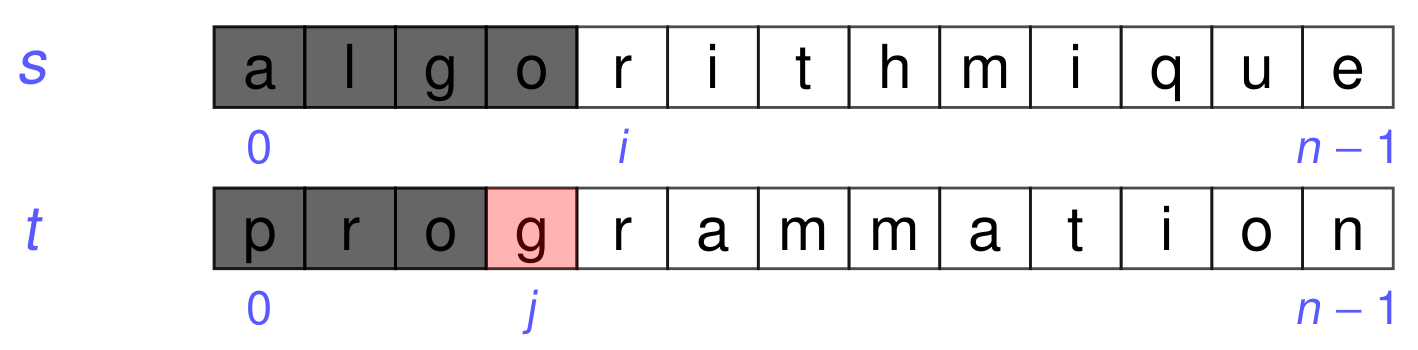
\includegraphics[width=0.8\textwidth]{progDyn_PLSC_schema1.png}
\caption{Représentation du problème de recherche de la plus longue séquence commune à deux chaînes de caractères $s$ et $t$.}
\label{fig:progDyn_PLSC_schema1}
\end{figure}
\item \textbf{Récurrence.} \\
Soit $L_{ij}$ la longueur de la PLSC pour $s[i:n-1]$ et $t[j:n-1]$. Si $s[i]=t[j]$, alors
$$L_{ij} = 1+ L_{i+1 \; j+1}$$, où $+1$ correspond à l'ajout de la lettre commune. \\

Si $s[i] \neq t[j]$, alors les deux cas sont possibles : $\left\{\begin{array}{l}
L_{i+1 \; j} \\ L_{i \; j+1}
\end{array} \right.$ et celui qui sera pris est celui qui maximise la longueur de la PLSC. \\

$$\boxed{L_{ij} = \left\{ \begin{array}{lr}
1+ L_{i+1 \; j+1} & \text{si} \; s[i]=t[j] \\
\max\{L_{i+1 \; j}\; , \quad L_{i \; j+1}\} & \text{sinon}
\end{array}\right. }$$
Le cas de base correspond au cas où un des deux indices est $n$, quand une des deux chaînes est vide. 

$$\boxed{\text{Cas de base : } \qquad L_{in} = L_{nj} = 0 \quad \forall \; i\; , i}$$
Et les coûts par sous-problèmes sont constants parce que nous considérons que tout a déjà été mémoïsé. \\

\item \textbf{Graphe de dépendance.}  \\
Nous pouvons dresser pour cela un tableau bidimensionnel. La question est "qu'est-ce qui dépend de quoi ?". Nous savons que $L_{ij}$ dépend de $L_{i+1\; j+1}$, $L_{i+1 \; j}$ et $L_{i \; j+1}$, mais tous les éléments ont cette même structure de dépendance. Il faut enfin construire l'ordre topologique en regardant d'où partent les flèches : il s'agit d'en bas à droite,c'est de là que doit partir la première flèche. Attention : plusieurs ordres topologiques peuvent marcher, bien entendu ! \\
\begin{figure}
\centering
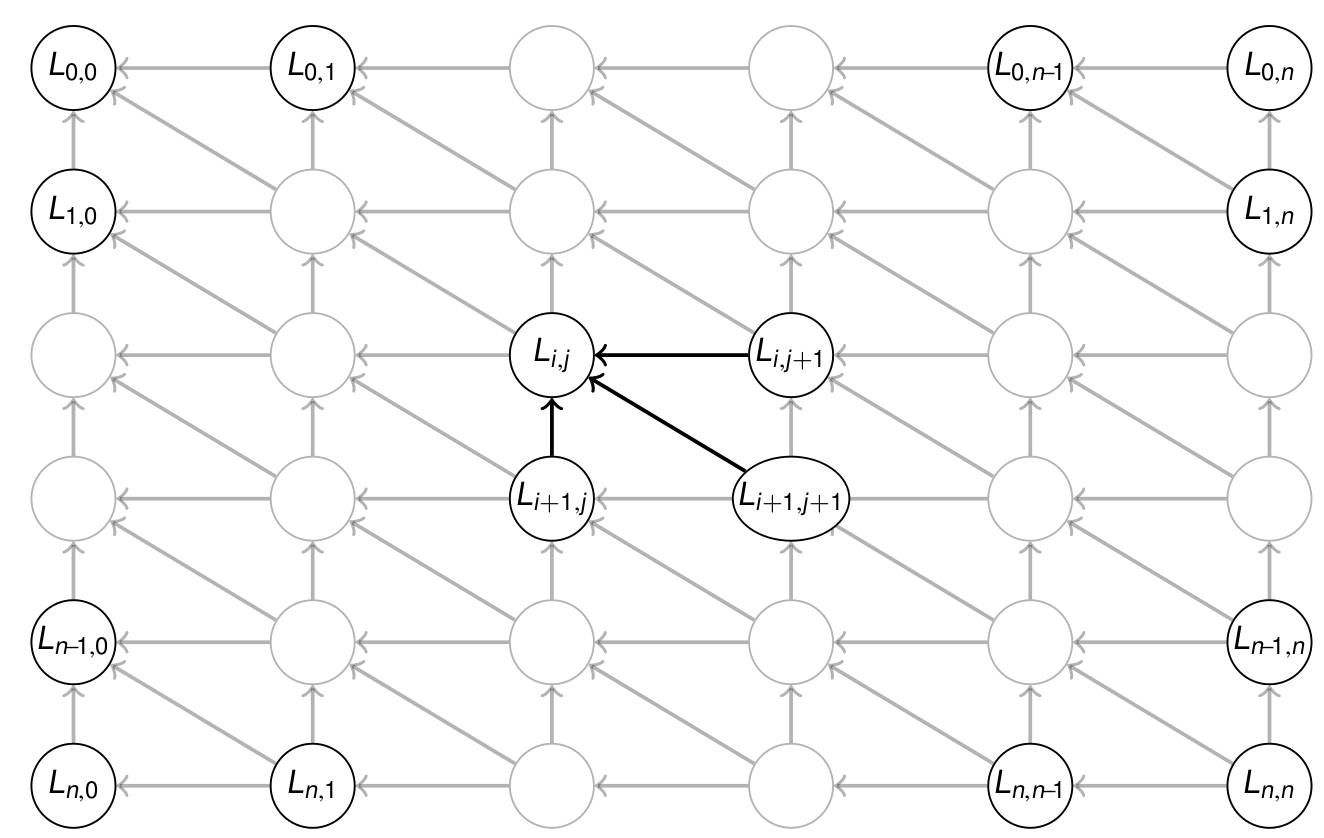
\includegraphics[width=0.9\textwidth]{progDyn_PLSC_graphe_dependance.png} \\
\vspace{1cm}
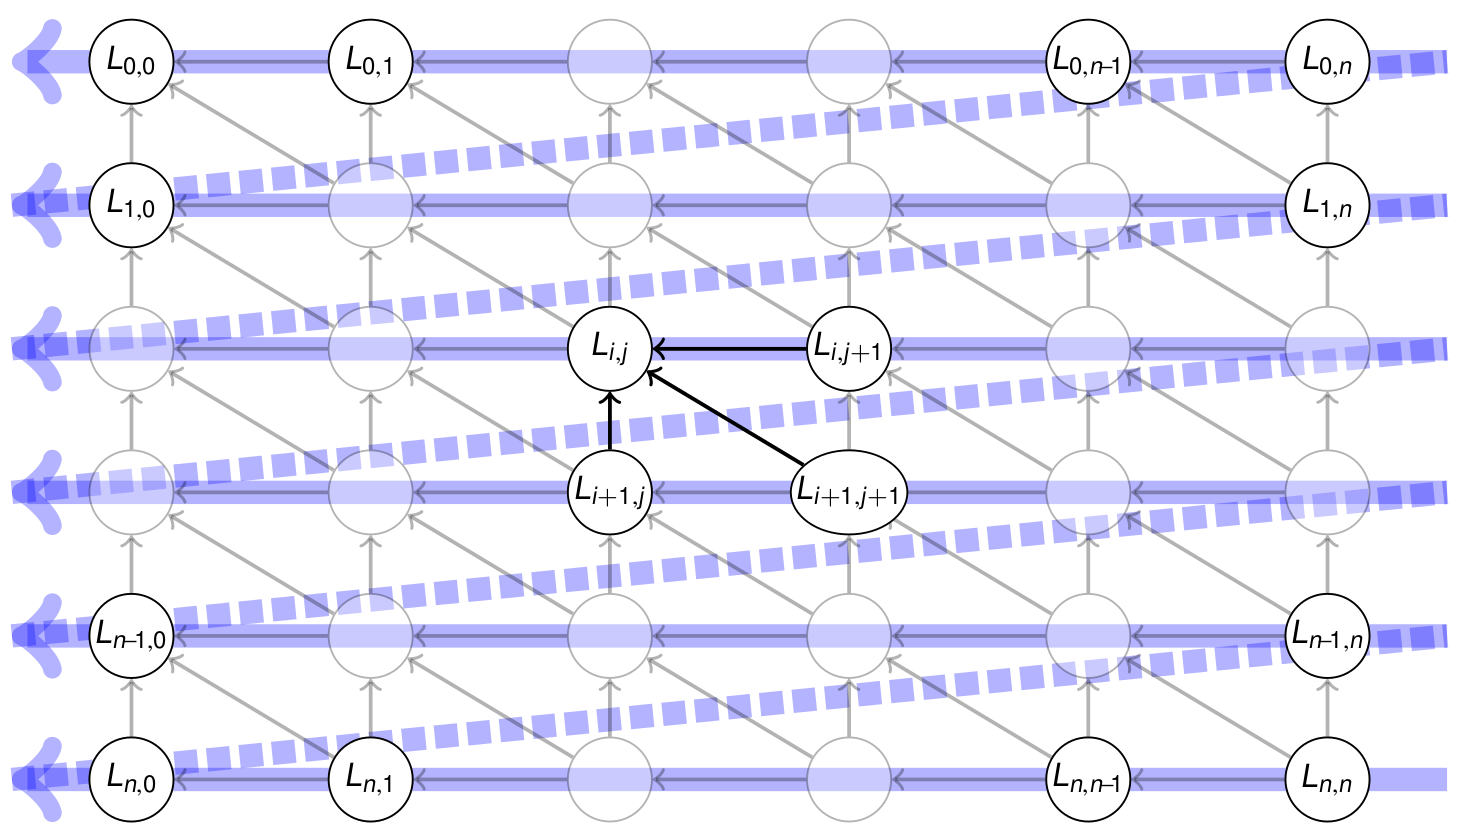
\includegraphics[width=0.9\textwidth]{progDyn_PLSC_graphe_dependance_2.png}
\caption{Graphe de dépendance et ordre(s) topologiques du problème de PLSC.}
\label{fig:progDyn_PLSC_graphe_dependance}
\end{figure}

\item \textbf{Problème initial.} \\
C'est lorsque les deux chaînes sont complètes : $L_{00}$. La détermination du coût total revient donc à prendre le nombre de sous-problèmes, le coût par sous-problème, et le coût additionnel pour le problème initial (une fois tous les sous-problèmes calculés, le problème initial est lui-même un des sous-problèmes et la valeur se trouve déjà en table de mémoïsation) : $\Theta(n^2) + \Theta(1) + \Theta(1) = \Theta(n^2)$. Remarque : si on essayait ça en recherche exhaustive on aurait un coût exponentiel.
\end{enumerate} 
\section{Démultiplication des sous-problèmes}
Comme on l'a déjà vu, il est très typique que l'input d'un problème soit un tableau. On va voir ici comment choisir les bons sous-tableaux lorsque l'input du problème est un tableau. 
\subsection{Approche générale}
L'approche générale consistait à considérer les suffixes, les préfixes ou les sous-tableaux. Cette approche ne marche pas toujours, parce qu'en construisant une solution candidate partielle, on se retrouve en effet avec un sous-problème similaire au problème initial, \textbf{mais avec des paramètres différents}. L'input est encore un tableau mais un (ou plusieurs) paramètre a changé. \\

Nous allons alors \textbf{définir un sous-problème par valeur possible des paramètres} : il s'agit de la \textbf{démultiplication des sous-problèmes}.

\bb{Démultiplication des sous-problèmes : un sous-problème par valeur possible des paramètres}
\subsection{Exemples}
\begin{itemize}
\item Pour le problème de pavage, comme on fait deux choix différents à chaque étape, on se retrouve à chaque étape avec deux versions du sous-problème : la version avec le côté gauche bleu et l'autre avec rouge.
\item Variante du problème du sac : chaque objet a un volume et une valeur. Et soit le problème d'optimisation de la \textbf{valeur du sac} et non le volume. On va l'étudier en détail.
\end{itemize}
\subsubsection{Variante du problème du sac}
On peut dire qu'à chaque choix, on se retrouve avec un suffixe, mais le volume dans le sac est plus petit ! Donc on voudra maximiser la valeur du sac mais avec un volume disponible plus petit : le \textbf{volume disponible} qui est le paramètre. On démultiplie donc les sous-problèmes selon $v$ le volume disponible. \\

Après démultiplication, nous avons donc les sous-problèmes suivants, notés $K_{iv}$ :
\begin{itemize}
\item Pour chaque paramètre $v$, on a les $n$ suffixes car $i = 0 \longrightarrow n-1$
\item Le paramètre $v$ varie de $0$ à $V$ : $0\leq v \leq V$.
\item[$\Rightarrow$] \# sous-problèmes : $\Theta(n\cdot V)$.
\end{itemize}
La \bleu{\textbf{troisième étape}} consiste à évaluer $K_{iv}$ pour obtenir une récurrence : faire le meilleur choix possible à chaque étape. Pour atteindre $K_{iv}$, il faut soit prendre $i$ soit non, et résoudre le sous-problème restant de manière optimale. Si on prend $i$, alors la valeur du sac augmente de $\text{Val}[i]$ et le volume diminue de $\text{Vol}[i]$. 

$$\boxed{K_{iv} = \left\{ \begin{array}{lr}
\max\{K_{i+1 \; v}\; , \quad K_{i+1 \; v-\text{Vol}[i]} + \text{Val}[i]\} &\text{Si } \; \text{Vol}[i] \leq v \\
K_{i+1 \; v} & \text{Sinon}
\end{array} \right. }$$
Le cas de base correspond à un cas $K_{nv}$ qui est nul pour tout volume restant parce qu'il n'y a plus aucun objet à considérer. \\

Le coût par sous-problème est constant parce qu'on consière que tout a été mémoïsé. \\

La \textbf{\bleu{quatrième étape}} est le graphe de dépendance : $K_{iv}$ dépend de $K_{i+1 \; v}$ et des $K{i+1 \; w}$ où les $w$ sont des volumes inférieurs à $v$. On commence donc à la première ligne du graphe et puis on remonte : voilà l'ordre topologique. Sur la première ligne on peut calculer tous les éléments indépendamment, on peut donc proposer un ordre topologique qui calcule de gauche à droite en remontant à chaque ligne. \\

\begin{figure}[h]
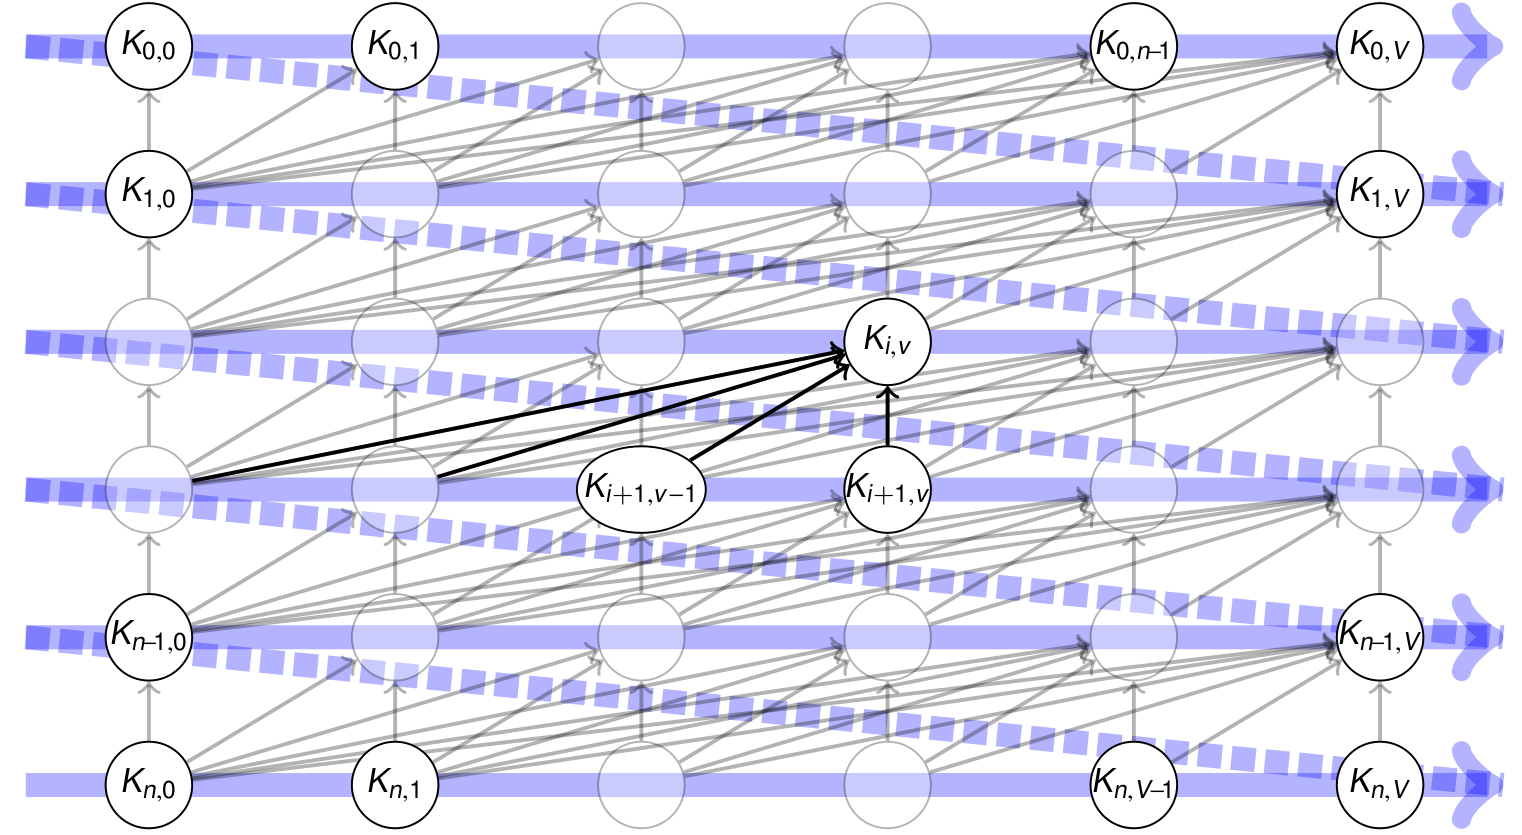
\includegraphics[width=\linewidth]{progDyn_demult_graphe_dep.png}
\caption{Graphe de dépendance pour la variante du problème de sac à dos, abordée par la programmation dynamique.}
\label{fig:progDyn_demult_graphe_dep}
\end{figure}

La \textbf{\bleu{cinquième étape}} concerne le problème initial : il faut résoudre tous les problèmes puis calculer la valeur pour le problème initial. Mais si tout a déjà été calculé, le coût additionnel est un temps constant, donc, avec $\Theta(n\cdot V)$ sous-problèmes et $\Theta(1)$ comme coût pour chaque sous-problème, nous avons un coût total de $\Theta(n \cdot V)$. \\

C'est une complexité \textbf{pseudo-polynomiale} parce qu'il y a un autre paramètre apparaît, et que ce facteur est la \textbf{valeur maximale des entiers définissant le problème}. C'est mieux qu'une complexité exponentielle mais c'est moins bon qu'une complexité polynomiale.
\section{Algorithmes gloutons}
Nous allons faire un retour en arrière et discuter des algorithmes gloutons. Contrairement à la programmation dynamique, on n'arrive pas ici à une solution optimale, mais une complexité souvent plus petite. \\

\subsection{Comparaison glouton -- progDyn}
En programmation dynamique, à chaque étape il faut choisir entre plusieurs possibilités. On s'assure de prendre le choix qui \textbf{mène à une solution optimale}. On a pour ça besoin de la récursion pour aller voir plus loin. \\

Avec un algorithme glouton, face à un choix, on choisit directement la possibilité qui \textbf{semble être la meilleure}. Ils sont souvent simples et rapides, mais ne mènent pas toujours ) une solution optimale. Alors, si on préfère proditer du gain en temps de calcul et qu'une solution sous-optimale est acceptable, alors on \textbf{peut utiliser un algorithme glouton}. Une autre possiblite d'utiliser un algorithme glouton est si on arrive à prouver qu'on peut arriver à une solution optimale.

\subsection{Exemple du problème du sac-à-dos}

\end{document}